% Style for a MSc paper at Warsaw School of Economics
% Michał Ramsza
% Friday, December 14, 2012

% --- document class and other global stuff ---------------------------
\documentclass[polish, twoside, 12pt, a4paper]{article}

% --- packages --------------------------------------------------------
\usepackage{textcomp}
\usepackage{times}
\usepackage{amsmath}
\usepackage{amsfonts}
\usepackage{amssymb}
\usepackage{amsthm}
\usepackage[T1]{fontenc}
\usepackage[utf8]{inputenc}
\usepackage{graphicx}
\usepackage{xcolor}
\usepackage{enumitem}
\usepackage[polish]{babel}
\usepackage[centering, left=3.5cm, right=2.5cm, textheight=24cm]{geometry}
\usepackage{gensymb}
\usepackage{float}
% --- packages for citations ------------------------------------------
\usepackage{natbib}
\AtBeginDocument{\renewcommand{\harvardand}{i}}

% --- package for automatic insertion of R code -----------------------
\usepackage{listings}
\lstset{language=R,%
   numbers=left,%
   tabsize=3,%
   numberstyle=\footnotesize,%
   basicstyle=\ttfamily \footnotesize \color{black},%
   escapeinside={(*@}{@*)}}

% --- support for links -----------------------------------------------	
\usepackage{url}
\usepackage{hyperref}
\hypersetup{colorlinks=true,
            linkcolor=black,
            citecolor=darkgray,
            urlcolor=darkgray,
            pagecolor=darkgray}

% --- support for large tables and other stuff ------------------------	
\usepackage{longtable}
%\usepackage{subfigure} % this package will now work with subcaption package
\usepackage{float}
\usepackage{caption}
\usepackage{subcaption}


% --- definitions for environments -------------------------------------
\theoremstyle{definition}
    \newtheorem{condition}{Assumption}
    \newtheorem{example}{Example}      

\theoremstyle{plain}
    \newtheorem{definition}{Definition}    
    \newtheorem{proposition}{Proposition}
    \newtheorem{theorem}{Theorem}
    \newtheorem{cor}{Corollary}

\theoremstyle{remark}
    \newtheorem{remark}{Remark}

% --- other settings --------------------------------------------------
\linespread{1.5}
\frenchspacing
\sloppy
\allowdisplaybreaks[4]
\raggedbottom
\clubpenalty=10000
\widowpenalty=10000

% --- only if required ------------------------------------------------
\AtBeginDocument{\renewcommand*{\figurename}{Wykres}}
\AtBeginDocument{\renewcommand*{\tablename}{Tabela}}

% ---------------------------------------------------------------------
\begin{document}

% --- strona tytulowa -------------------------------------------------
\begin{titlepage}
\centering


\includegraphics[width=0.66\textwidth]{logo.JPG}

\vspace*{0.5cm}
Studium licencjackie\\
\begin{flushleft}
Kierunek: Metody Ilościowe w Ekonomii i Systemy Informacyjne\\
Specjalność: Metody Analizy Decyzji\\
Forma studiów: stacjonarne
\end{flushleft}

\vspace*{.5cm}
\rule{0cm}{1cm}\hfill
\begin{minipage}{9cm}
Imie i nazwisko: Michał Cisek\\
Nr albumu: 56283
\end{minipage}

\vspace*{1cm}
\begin{minipage}{12cm}
\centering
\Large
\textbf{Wyznaczenie reguł asocjacyjnych \\ z finansowych szeregów czasowych \\ na przykładzie indeksu giełdowego WIG20}
\end{minipage}

\vspace*{2cm}
\rule{0cm}{1cm}\hfill
\begin{minipage}{9cm}
Praca licencjacka napisana\\
w Kolegium Analiz Ekonomicznych\\
w Katedrze Matematyki i Ekonomii Matematycznej\\
pod kierunkiem naukowym\\
dr hab. Michała Ramszy
\end{minipage}

\vfill
Warszawa 2015
\end{titlepage}

\rule{1ex}{0ex}\clearpage


% --- table of contents -----------------------------------------------
\cleardoublepage
\tableofcontents

% --- chapter ---------------------------------------------------------
\cleardoublepage
\section{Wprowdzenie}

Analiza techniczna koncentruje się na badaniu zachowań rynku, głównie poprzez analizę wykresów oraz wolumenu zawartych transakcji. Propagatorzy tej teorii powołują się
na 3 reguły (\cite{Murphy1999}). Pierwsza z nich zakłada, że rynek dyskontuje wszystko. Oznacza to, że każda informacja, zarówno ekonomiczna, polityczna czy gospodarcza, mogąca wpłynąć na cenę danej akcji czy innego
instrumentu finansowego, ma w nim pełne odzwierciedlenie. Druga teza stanowi, iż ceny podlegają trendom, tzn. wykazaują  tendencję do poruszania się w jednym kierunku. W analizie technicznej 
wszystkie ruchy cen, w różnym zakresie czasowym klasyfikowane są na trendy spadkowe, wzrostowe i horyzontalne. Teza ta jest przeciwstawna do teorii stanowiącej o tym, że notowania rynków finansowych 
poruszają się zgodnie z procesem błądzenia losowego. Takie stwierdzenie zaprzecza istnieniu takiego pojęcia jak trend, ponieważ implikuje ono, iż poprzednie ruchy cen nie wpływają na jej przyszłe zachowania. 
Ostatnim założeniem analizy technicznej jest pogląd, że historia się powtarza. Stanowisko to wywodzi się z faktu, iż analiza bada zachowanie rynku, który tworzony jest przez wielu inwestorów. Badanie rynku
sprowadza się więc do badania zachowań ludzi w różnych sytuacjach rynkowych, a te pozostają niezmienne i dlatego możemy wyciągać wnioski z przeszłych notowań rynku. 

Zarzutów wobec analizy technicznej na przestrzeni lat pojawiało się wiele. Jako przykład można podać wyżej wspomniane dyskusje na temat faktu istnienia trendów na rynkach finansowych. Dodatkowo powstawało wiele 
opracowań sugerujących bezużyteczność tej metody do celów inwestycyjnych. Rozbieżność zdań w tej kwestii jest jednak spora. Niektóre badania sugerują bezwartościowość ponad 5 tysięcy reguł
stosowanych w analizie technicznej, wskazując jednocześnie że lepsze zastosowania mogą mieć na rynkach wschodzących niż na rozwiniętych. Twórcy innych artykułów sugerują natomiast, że użycie nawet tak 
prostych narzędzi analizy technicznej jak np. średnia ruchoma potrafi przynosić lepsze rezultaty niż przy użyciu takich modeli szeregów czasowych jak model autoregresyjny (AR), GARCH bądź EGARCH.  

Poza wskaźnikami i oscylatorami, jednym z podstawowych narzędzi analizy technicznej są formacje cenowe, czyli pewne powtarzające się układy cenowe występujące sekwencyjnie w czasie, używane 
do przewidywania przyszłych ruchów notowań. Formacje klasyfikowane są na te sygnalizujące odwrócenie panującego trendu oraz na te zwiastujące jego kontynuację. Powodem popularności tego narzędzia 
jest przede wszystkim prostota, a także łatwość dostępu do opisu wszystkich formacji, które można znaleźć zarówno w internecie, jak i innych źródłach (\cite{Bulkowski2005}). Rodzi to jednak pewne problemy. Głównym
z nich jest subiektywność i dwuznacznaczność formacji. John J. Murphy w książce Analiza techniczna rynków finansowych zacytował Richarda Teweles, który określił, że formacje widoczne na wykresach są tworem niemal 
całkowicie subiektywnym i że nikomu nie udało się dotychczas poddać ich matematycznej kwantyfikacji. Dlatego też czytając analizy przygotowywane przez specjalistów z różnych domów maklerskich często można natrafić 
na spore rozbieżności dotyczące prognoz cen tego samego instrumentu finansowego. Bierze się to z wcześniej wspomnianej niejasności w interpretacji wykresu cen, ponieważ dla jednego analityka dana sekwencja będzie 
odbierana przykładowo jako formacja głowy z ramionami (formacja odwrócenia trendu), natomiast drugi odczyta ją jako formacje klinu (formacja kontynuacji trendu).

Podsumowując rozważania na temat przydatności analizy technicznej, możemy stwierdzić że niewątpliwą zaletą jest prostota rozpoczęcia inwestycji za jej pomocą (do korzystania z wielu metod analizy technicznej, 
tj. Price Action potrzebny jest tylko dostęp do wykresu notowań), a także mnogość publikacji dotyczących opisu i oceny jej narzędzi. Trzeba jednak zauważyć także spore zarzuty, szczególnie jeśli chodzi o zastosowanie
podstawowego narzędzia analizy technicznej, czyli formacji cenowych. Chcąc więc wydobyć pewne powtarzające się schematy, które niosłyby ze sobą pewną prognostyczną wartość, prawdopodobnie najlepszym rozwiązaniem 
byłoby użycie narzędzi data miningu. Na przestrzeni ostatnich lat powstało wiele artykułów (\cite{Akkaya2011},  \cite{Zhang2004}, \cite{Weigend1996}) potwierdzających rosnącą rolę tej interdyscyplinarnej dziedziny nauki w zastosowaniach finansowych, głównie 
dzięki temu, że w sprawny sposób możliwe jest wyciągnięcie wartościowych informacji z dużych zbiorów danych. Ponadto możliwe jest uzyskanie reguł asocjacyjnych, które pomagają w odkryciu związków w pozornie 
nieskorelowanych danych.  Celem tej pracy jest zastosowanie własnego algorytmu, korzystającego m.in. właśnie z mechanzmów data minigu i metod statystycznych do ekstrakcji takich formacji  z finansowego szeregu czasowego, 
dzięki którym przy ponownym pojawieniu będziemy w stanie z wysokim prawdopodobieństwem przewidzieć przyszły ruch cen. Dokonana zostanie także ocena użytego algorytmu. 


% --- chapter ---------------------------------------------------------
\clearpage
\section{Metodologia}

Finansowe szeregi czasowe głównie z powodu niestacjonarności, wrażliwości na małe zmiany oraz zawierania w sobie dużej ilości
szumów są problematyczne w prognozowaniu. Aby dokonać wyciągnięcia pewnych zależności z nich, należy przejść przez pewne etapy, w których dochodzi do obróbki i  przygotowania danych.  W literaturze znajduje się wiele artykułów poświęconych tej tematyce. 
Przykładowo \cite{Dante2010} starają się odszukać korelacji w ruchach cen między spółkami wchodzącymi w skład indeksu giełdowego w Madrycie (Madrid Stock Exchange General Index). W tym celu użyty zostaje algorytm ECLAT. Zanim jednak zostaje 
on zastosowany, następuje wygładzanie szeregu czasowego metodą Gaussian Kernel Smoothing. Jest to wygładzanie podobne do użycia arytmetycznej średniej ruchomej. W tym przypadku jednak, starsze obserwacje są mniej istotne przy obliczaniu 
średniej. Dodatkowo wagi dla starszych obserwacji rozłożone są zgodnie z funkcją Gaussa (\url{http://bossafx.pl/fx/narzedzia/patterns-recognizer/obliczanie-formacji/}). W niektórych artykułach (\cite{Gandhmal2011}, \cite{Khan2011}, \cite{Aragianni2010}) dodana była faza 
klastrowania danych, najczęściej za pomocą metody k-średnich, bądź też Optymalizacji Stadnej Cząsteczek (Particle Swarm Optimization). W przypadku tych prac, do wygenerowania zbioru reguł użyto algorytmu CIR (Consistent Item set Rule algorithm), 
podobnego swym działaniem do algorytmu Apriori, a także algorytmu MFP (Most Frequent Pattern algorithm). Często też pojawiającą się koncepcją jest zastosowanie sieci neuronowych do prognozowania cen notowań (\cite{Kaastra1996}, \cite{Virili2001}). 

Pomimo wielu podejść do tego tematu, pewne schematy postępowania dla różnych artykułów są podobne. Z tego względu w dalszej części pracy opisane są szczegółowo kolejne kroki zaproponowanego przeze mnie algorytmu, zawierające techniki podobne 
do tych użytych w wyżej wspomnianych pracach.

\subsection{Czyszczenie danych}

Pierwszym etapem algorytmu jest wyczyszczenie danych za pomocą odpowiedniego filtra, tak aby z jednej strony ułatwić łatwiejsze rozpoznawanie trendów, ale z drugiej strony, żeby pierwotny szereg nie utracił swoich właściwości. Z pomocą przychodzą 
tutaj filtry pierwotnie stosowane jako układy elektroniczne do przetwarzania sygnału. Do ich grona można zaliczyć np.: filtr Hodricka-Prescotta czy Baxtera Kinga. Ich zadaniem jest oczyszczenie procesów ze wskazanych składników. Pierwszy z nich eliminuje 
trend długofalowy, podczas gdy drugi dokonuje eliminacji trendu wraz z cyklicznością (\cite{Kufel2005}). Kolejnym przykładem może być rodzina filtrów dolnoprzepustowych, do których należy przykładowo filtr Butterwortha. Głównym ich zadaniem jest 
przepuszczanie tylko tych częstotliwości sygnału pierwotnego, które są poniżej ustalonej częstotliwości granicznej. Dzięki temu możemy pozbyć się z szeregu szumów o dużej częstotliwości. Warto tutaj nadmienić, że występują one powszechnie praktycznie 
w każdym odbiorniku radiowym. 

Najczęstszym sposobem pozbywania się szumów z szeregu czasowego jest jednak zastosowanie jednej z metod wygładzania. Wyróżniamy tutaj m.in. metodę średniej, metodę ruchomej średniej, metodę ruchomej mediany oraz metodę wielomianu 
gładzącego (\cite{Huk2001}). Do tej ostatniej grupy należy filtr Savitzky'ego-Golaya. Zasada działania jest następująca. Dla podanej liczby punktów (liczba ta musi być nieparzysta) dopasowywany jest wielomian stopnia przez nas z góry określonego. 
Wartość tego wielomianu w punkcie środkowym jest elementem wygładzonym. To postępowanie wykonywane jest dla kolejnych punktów szeregu czasowego. Wzór (\ref{1}) przedstawia ogólne równanie na wartości wygładzone za pomocą tego filtra, 
gdzie \(a_{i}\) są współczynnikami dopasowania wielomianu, \(NP\) oznacza liczbę punktów wybranych do dopasowania wielomianu, a \(H\) jest normą. Tabela zawierająca współczynniki dopasowania wielomianu kwadratowego oraz odpowiednie normy 
znajduje się w Dodatku A 

\begin{equation}\label{1}
Y_{t}=\frac{1}{H}\sum_{i=-(NP-1)/2}^{(NP-1)/2} a_{i}x_{t+i}.
\end{equation}

\subsection{Segmentacja}

Po dokonaniu odpowiedniego czyszczenia danych, należy przeprowadzić segmentację szeregu. Głównym motywem przyświecającym temu zadaniu jest znaczące przyspieszenie działania algorytmu wyznaczania reguł asocjacyjnych. Należy jednak dokonać tego za pomocą takiego narzędzia, które pozwoli na jak najlepsze zebranie informacji o charakterystyce danego szeregu. 

Pierwszym proponowanym algorytmem jest algorytm segmentacji kawałkami liniowej (piecewise linear segmentation). Jednym ze sposobów zastosowania go jest użycie środowiska do obliczeń statystycznych R, a konkretnie funkcji \(linearSegmentation\) zawartej w pakiecie ifultools (\cite{ifultools}). Funkcja ta przyjmuje dwa argumenty: \(n.fit\) oraz \(angle.tolerance\). Pierwszy argument określa szerekość okien, na które dzielony jest szereg czasowy. Dla pierwszego okna dopasowywana jest prosta za pomocą metody najmniejszej kwadratów, a na jej podstawie wyliczany jest kąt nachylenia do osi odciętych. Następnie ten sam schemat powtarzany jest dla kolejnego okna i następuje porównanie kątów nachylenia. Jeśli różnica w nachyleniu prostych przekracza wielkość argumentu \(angle.tolerance\), wtedy punkt pomiędzy tymi oknami jest uznany jako punkt zmiany. W przeciwnym razie powstaje nowa prosta, powstała z połączenia dwóch okien. Kolejno nowo powstała prosta porównywana jest z sąsiednią i takie postępowanie przebiega sekwencyjnie aż do ostatniego okna.

Drugim podejściem zastosowanym w tej pracy jest użycie narzędzia, które dokona segmentacji szeregu w tych miejscach, gdzie zmianie ulegają pewne statystyczne własności (np. średnia czy wariancja). Istnieje kilka algorytmów, które tego dokonują, a mianowicie: Binary Segmentation, Segment Neighbourhoods oraz Pruned Exact Linear Time (PELT). Zasada działania tego pierwszego jest następująca:
\begin{enumerate}
  \item Przeprowadzany jest test statystyczny na istnienie pojedyńczego punktu zmiany (średniej lub wariancji). Jeśli punkt zmiany zostaje zidentyfikowany, dane dzielone są w tym miejscu na dwie części
  \item Procedura poszukiwania pojedyńczego punktu zmiany jest powtarzana dla obu części. W przypadku znalezienia tych punktów, dane są dalej dzielone
  \item Proces ten powtarzany jest do momentu, w którym w żadnej z części nie zostanie znaleziony punkt zmiany
\end{enumerate}
 
Algorytm ten jest popularny ze względu na szybkość obliczeń, jednak odbywa się to czasami kosztem dokładności znalezionych punktów.

Segment Neighbourhoods prezentuje przeciwne własności--- jest algorytmem dokładnym, ale o większej złożoności obliczeń.

Podczas gdy oba powyższe algorytmu stanowią pewien rodzaj kompromisu pomiędzy szybkością, a dokładnością, Pruned Exact Linear Time łączy ich mocne strony. Dzięki temu wyszukane punkty zmiany są wyznaczone precyzyjnie, a dzięki zastosowaniu dynamicznego programowania, algorytm jest efektywny obliczeniowo.

Do zastosowania powyższych algorytmów zastosowano funkcję \(cpt.mean\) z pakietu changepoint (\cite{changepoint}), która w zależności od wybranej metody przyjmuje odpowiedni argument \(method\) (\(``PELT"\) dla Pruned Exact Linear Time, \(``BinSeg"\) dla Binary Segmentation, \(``SegNeigh"\) dla Segment Neighbourhoods). Ponadto funkcja ta pozwala na specyfikacje odpowiedniej funkcji, która będzie zapobiegać zbytniemu dopasowaniu (sytuacji, w której punktów zmiany byłoby zbyt dużo). Dostępne funkcje kary to przede wszystkim kryteria informacyjne (Schwarza, Hannana-Quinna, Akaike'a), ale można ją także zdefiniować samemu. Za wybór odpowiedniego testu statystycznego odpowiada argument \(test.stat\), przyjmujący wartość \(``Normal"\), w przypadku gdy nasze dane mają rozkład normalny, lub \(``CUSUM"\) w przeciwnym wypadku.

Po dokonaniu segmentacji, zarówno za pomocą funkcji \(linearSegmentation\), jak i \(cpt.mean\) dokonane zostanie połaczenie tych segmentów, w których trend (wzór (\ref{2})) jest podobny. Taka procedura jest zastosowana, w celu ograniczenia tych fragmentów szeregu, które mają porównywalną charakterystyke

\begin{equation}\label{2}
Trend_{i}=\frac{y_{t}-y_{t-1}}{y_{t-1 }}*100.
\end{equation}

W tym celu zaimplementowałem własną funkcję \(MergeSimilarTrends\), której kod znajduje się ponizej. Przyjmuje ona 3 argumenty:
\begin{itemize}
  \item szereg - dane szeregu czasowego 
  \item changepoints - wektor zawierający miejsca punktów zmiany
  \item threshold - próg, poniżej którego sąsiednie segmenty są łączone
\end{itemize}

\begin{lstlisting}[language=R]
MergeSimilarTrends<-function(szereg,changepoints,threshold){

  changepoints[length(changepoints)+1]<-length(szereg)
  changepoints1<-c(rep(NA,length(changepoints)+1))
  changepoints1[2:length(changepoints1)]<-changepoints
  changepoints1[1]<-1
  changepoints<-changepoints1
  
  df<-data.frame(changepoint=changepoints,close=szereg[changepoints])
  
  trend<-rep(NA,length(changepoints))
  trend[1]=((df[1,2]-szereg[1])/szereg[1])*100
  for (i in 2:length(changepoints)){
    trend[i]=(((df[i,2]-df[i-1,2])/df[i-1,2])*100)
  }
  df<-data.frame(df,trend)
  
  similar<-rep(NA,length(changepoints))
  similar[1]='F'
  for (i in 2:length(changepoints)){
    ifelse(abs(df[i,3]-df[i-1,3])<=threshold,similar[i]<-'T',similar[i]<-'F')
  }
  df<-data.frame(df,similar)
  df$similar<-as.character(similar)
  
  rows_to_delete<-which(grepl('T',df$similar))-1
  df1<-df[-c(rows_to_delete),-c(3,4)]
  
  trend1<-rep(NA,length(df1[,1]))
  trend1[1]=((df1[1,2]-szereg[1])/szereg[1])*100
  for (i in 2:length(df1[,1])){
    trend1[i]=(((df1[i,2]-df1[i-1,2])/df1[i-1,2])*100)
  }
  df1<-data.frame(df1,Trend=trend1)
  
  DF<<-df1
  segmenty<<-df1$changepoint
}
\end{lstlisting}

\subsection{Symboliczna reprezentacja segmentów}

Posiadając podzielony szereg czasowy na segmenty o odpowiedniej charakterystyce trendu w nim panującego, oraz długości, należy dokonać budowy słownika, tak aby wyniki otrzymane z algorytmu użytego 
do wyznaczenia reguł asocjacyjnych były czytelne i łatwe w interpretacji.

Zakładając z góry, iż wiemy ile klas znajduje się w szeregu, moglibyśmy dokonać odpowiedniego podziału na podstawie histogramu czasu trwania fragmentów, oraz trendu, dobierając te parametry według własnej opinii. 
Takie postępowanie byłoby jednak subiektywne i mogłoby prowadzić końcowo do błędnych wniosków.

Biorąc to pod uwagę, racjonalnym pomysłem byłoby użycie jednego z narzędzi analizy skupień. \cite{BiecekPrzemysawTrajkowski2011} określił ją jako zbiór metod pozwalajacych na wyróznienie zbiorów 
obserwacji (nazywanych skupieniami lub klastrami) podobnych do siebie. Procedura podziału na zbiory nazywana jest grupowaniem bądź klasteryzacją. 

Jak wspominałem wcześniej we wprowadzeniu do tego rozdziału, często stosowanym w podobnych pracach narzędziem jest metoda k-średnich. Dokonuje ona podziału zbioru na zadaną ilość grup, a dokładniej rzecz ujmując, 
wyznacza współrzędne punktów, które będą środkami klastrów. Dany segment będzie należał do tego zbioru, którego środek znajduje się w najmniejszej odległości od niego.


\subsection{Rule extraction}

Po skończonej fazie przygotowania danych, przychodzi kolej na ich eksplorację, czyli uzyskanie użytecznych informacji. Jedną z najpopularniejszych metod eksploracji jest metoda asocjacyjna (metoda odkrywania asocjacji), 
która polega na przeszukiwaniu rekordów bazy danych w celu znalezienia w niej powtarzających się zależności. Stosuje się ją tam, gdzie występuja potrzeba scharakteryzowania związków przyczynowo-skutkowych pomiędzy danymi. 
 
Istnieją dwie miary określające reguły asocjacyjne: wsparcie (support), oraz pewność (confidence). 
Wsparcie jest parametrem, który określa jaki procent wszystkich reguł asocjacyjnych stanowi ta wybrana reguła.
Pewność reguły stanowi jaki procent transakcji zawartych w lewej stronie reguły prowadził do prawej strony. Wzory (\ref{3}) oraz (\ref{4}) przedstawiają 
formalny zapis powyższych parametrów
\begin{equation}\label{3}
wsparcie=P(A\ \cap B)=\frac{liczba\ transakcji\ zawierajacych\ A\ i\ B}{calkowita\ liczba\ transakcji},
\end{equation}

\begin{equation}\label{4}
pewnosc=P(B\ |\ A)=\frac{P(A\ \cap B)}{P(A)}=\frac{liczba\ transakcji\ zawierajacych\ A\ i\ B}{liczba\ transakcji\ zawierajacych\ A}.
\end{equation}

W opracowaniach znajduje się wiele algorytmów, służących generowaniu reguł asocjacyjnych, które powinny dawać podobne rezultaty, jednak 
różnią się efektywnością obliczeniową. Na potrzeby tej pracy, użyty zostanie najpopularniejszy algorytm Apriori.

Swoje działanie uzasadnia na podstawie własności funkcji wsparcia, która mówi, że powiększenie zbioru nieczęstego (zbioru zdarzeń, który występuje rzadziej niż 
zadane przez użytkownika minimalne wsparcie) o dodatkowe składowe nie spowoduje utworzenia zbioru częstego. Innymi słowy, w każdej iteracji tego algorytmu, odrzucane są 
te zbiory, dla których wsparcie jest niewystarczające. Powiększane są natomiast zbiory częste, do momentu kiedy jest to możliwe.

\subsection{Ocena jakości algorytmu}

Ostatnim elementem jest ocena tego, jak znalezione przez algorytm asocjacje sprawdzają się do prognozowania. W tym celu zbiór danych podzielony zostanie na dwie części: zbiór treningowy i zbiór testowy. Na 
pierwszym z nich dokonywana jest faza uczenia, tzn. generowane są na nim reguły asocjacyjne. W drugiej fazie, zwanej fazą testowania, następuje weryfikacja dokładności wyznaczonych asocjacji. Dokładniej rzecz 
ujmując, na zbiorze testowym wyszukiwane są lewe strony reguł, a następnie sprawdzane jest czy następny segment pokrywa się z tym zawartym w asocjacji. Na tej podstawie wyliczany jest współczynnik 
dokładności (wzór (\ref{5})), stanowiący procent wszystkich poprawnie zakwalifikowanych przypadków.

Ocena trafności prognostycznej wyznaczonych reguł zwana jest często sprawdzianem krzyżowym. Pozwala uniknąć ona tzw. błędu trzeciego rodzaju. Bez jego użycia, niemożliwe jest określenie czy wyznaczone reguły 
będą działały równie dobrze dla danych, nie użytych to ich konstrukcji. Jeśli dane asocjacje będą sprawdzały się równie dobrze na zbiorze treningowym i testowym, wtedy określa się, żę zbiór reguł pozytywnie przeszedł 
sprawdzian krzyżowy

\begin{equation}\label{5}
wspolczynnik\ dokladnosci= \frac{poprawnie\ zaklasyfikowane\ reguly}{wszystkie\ reguly\ ukazane\ w\ zbiorze\ testowym }.
\end{equation}

% --- chapter ---------------------------------------------------------
\clearpage
\section{Zastosowanie algorytmu \\ dla indeksu giełdowego WIG20}

Rozdział ten zawiera zastosowanie algorytmu opisanego we wcześniejszej części pracy, dla Warszawskiego Indeksu Giełdowego dwudziestu największych spółek notowanych na Giełdzie Papierów Wartościowych w 
Warszawie.

WIG20 jest indeksem giełdowym reprezentującym 20 największych i najpłynniejszych spółek notowanych na Giełdzie Papierów Wartościowych w Warszawie. Wyliczany jest od 16 kwietnia 1994 r., przyjmując poziom bazowy 
w wysokości 1000 punktów. Publikowany będzie do końca grudnia 2015 r., ponieważ zostanie docelowo zastąpiony przez indeks WIG30. Wzór (\ref{6}) przedstawia formułę pozwalającą wyliczyć indeks na daną chwilę. WIG20 jest indeksem cenowym, 
ponieważ bierzę pod uwagę tylko ceny zawartych transakcji (bez dywidend) przy kalkulacji. Skład tego indeksu ulega zmianie, kiedy dana spółka nie spełnia określonych wymogów (m.in. wymogów dotyczących liczby akcji w wolnym obrocie). 
Zmiany te dokonywane są podczas rewizji kwartalnych przeprowadzanych w trzeci piątek czerwca, września i grudnia, oraz podczas rewizji rocznej, dokonywanej w trzeci piątek marca

\begin{equation}\label{6}
WIG20(t)=\frac{M(t)}{M(0)*K(t)}*1000.
\end{equation}

Powodów, dla których warto użyć akurat tego indeksu, zamiast wielu innych, czy też innych instrumentów finansowych jest kilka:
\begin{itemize}
	\item pozwala śledzić koniunkturę w sektorze największych przedsiębiorstw,
	\item uznawany jest jako barometr sytuacji gospodarczej w kraju,
	\item stanowi podstawę do oceny wyników inwestycyjnych, zarówno dla inwestorów indywidualnych, jak i instytucjonalnych,
	\item jest instrumentem bazowym dla kontraktów terminowych i opcji notowanych na GPW.
\end{itemize}

Dane użyte w dalszej części pracy zostały pobrane z serwisu internetowego stooq.pl i zawierają wartości WIG20 pomiędzy 18 kwietnia 1994 r. a 8 maja 2015 r. (5235 obserwacji). Notowania indeksu w tym okresie przedstawia rysunek~\ref{rys001}.

\begin{figure}[H]
  \centering

  \begin{subfigure}[t]{1.00\textwidth}
    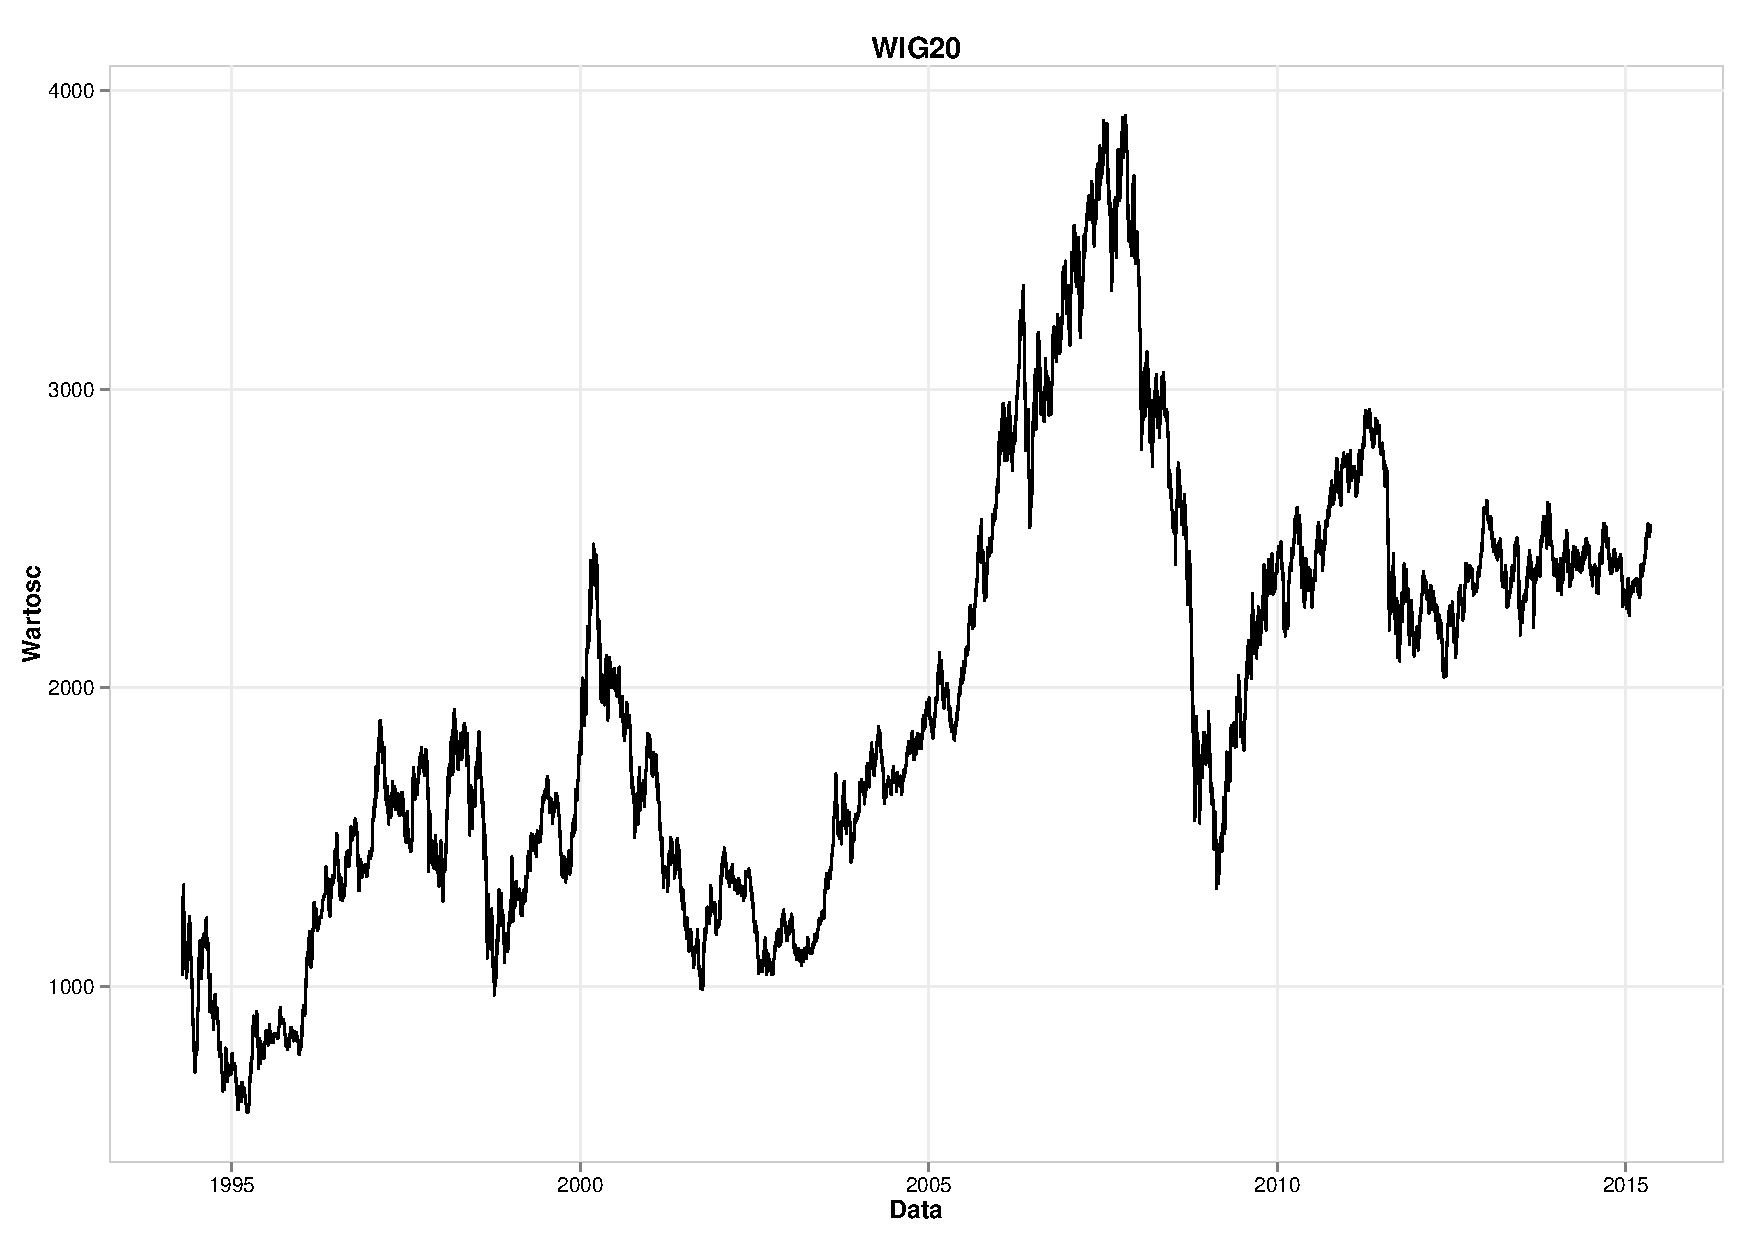
\includegraphics[width=\textwidth]{./rys001}
  \end{subfigure}

  \captionsetup{margin=10pt,font=small,labelfont=bf,width=.8\textwidth}

  \caption[WIG20 18.04.94 r. - 08.05.15 r.]{WIG20 18 kwietnia 1994 r. - 8 maja 2015 r. \textit{Źródło:} opracowanie własne}\label{rys001}
\end{figure}


\subsection{Czyszczenie danych filtrem Savitzky'ego-Golaya}

Łatwo można zauważyć na podstawie rysunku~\ref{rys001}, że notowania te zawierają wiele szumów, które uniemożliwiłyby poprawną klasyfikacje trendów w wybranych segmentach. Aby uniknąć tego problemu, zostanie użyty 
filtr Savitzky'ego-Golaya. Jak już wcześniej było wspomniane, określają go dwa parametry: stopień wielomianu użytego do filtracji, oraz liczba punktów użyta do oszacowania tego wielomianu. Należy tutaj jednak 
pamiętać, by dobrać te parametry tak, aby uzyskać kompromis pomiędzy wygładzaniem danych, a jak najwierniejszym oddaniem własności pierwotnego szeregu. Rysunek~\ref{rys017} przedstawia porównanie 
oryginalnego indeksu WIG20 wraz z 3 wykresami użycia filtru Savitzky'ego-Golaya dla różnych parametrów.

\begin{figure}[H]
  \centering

  \begin{subfigure}[t]{1.00\textwidth}
    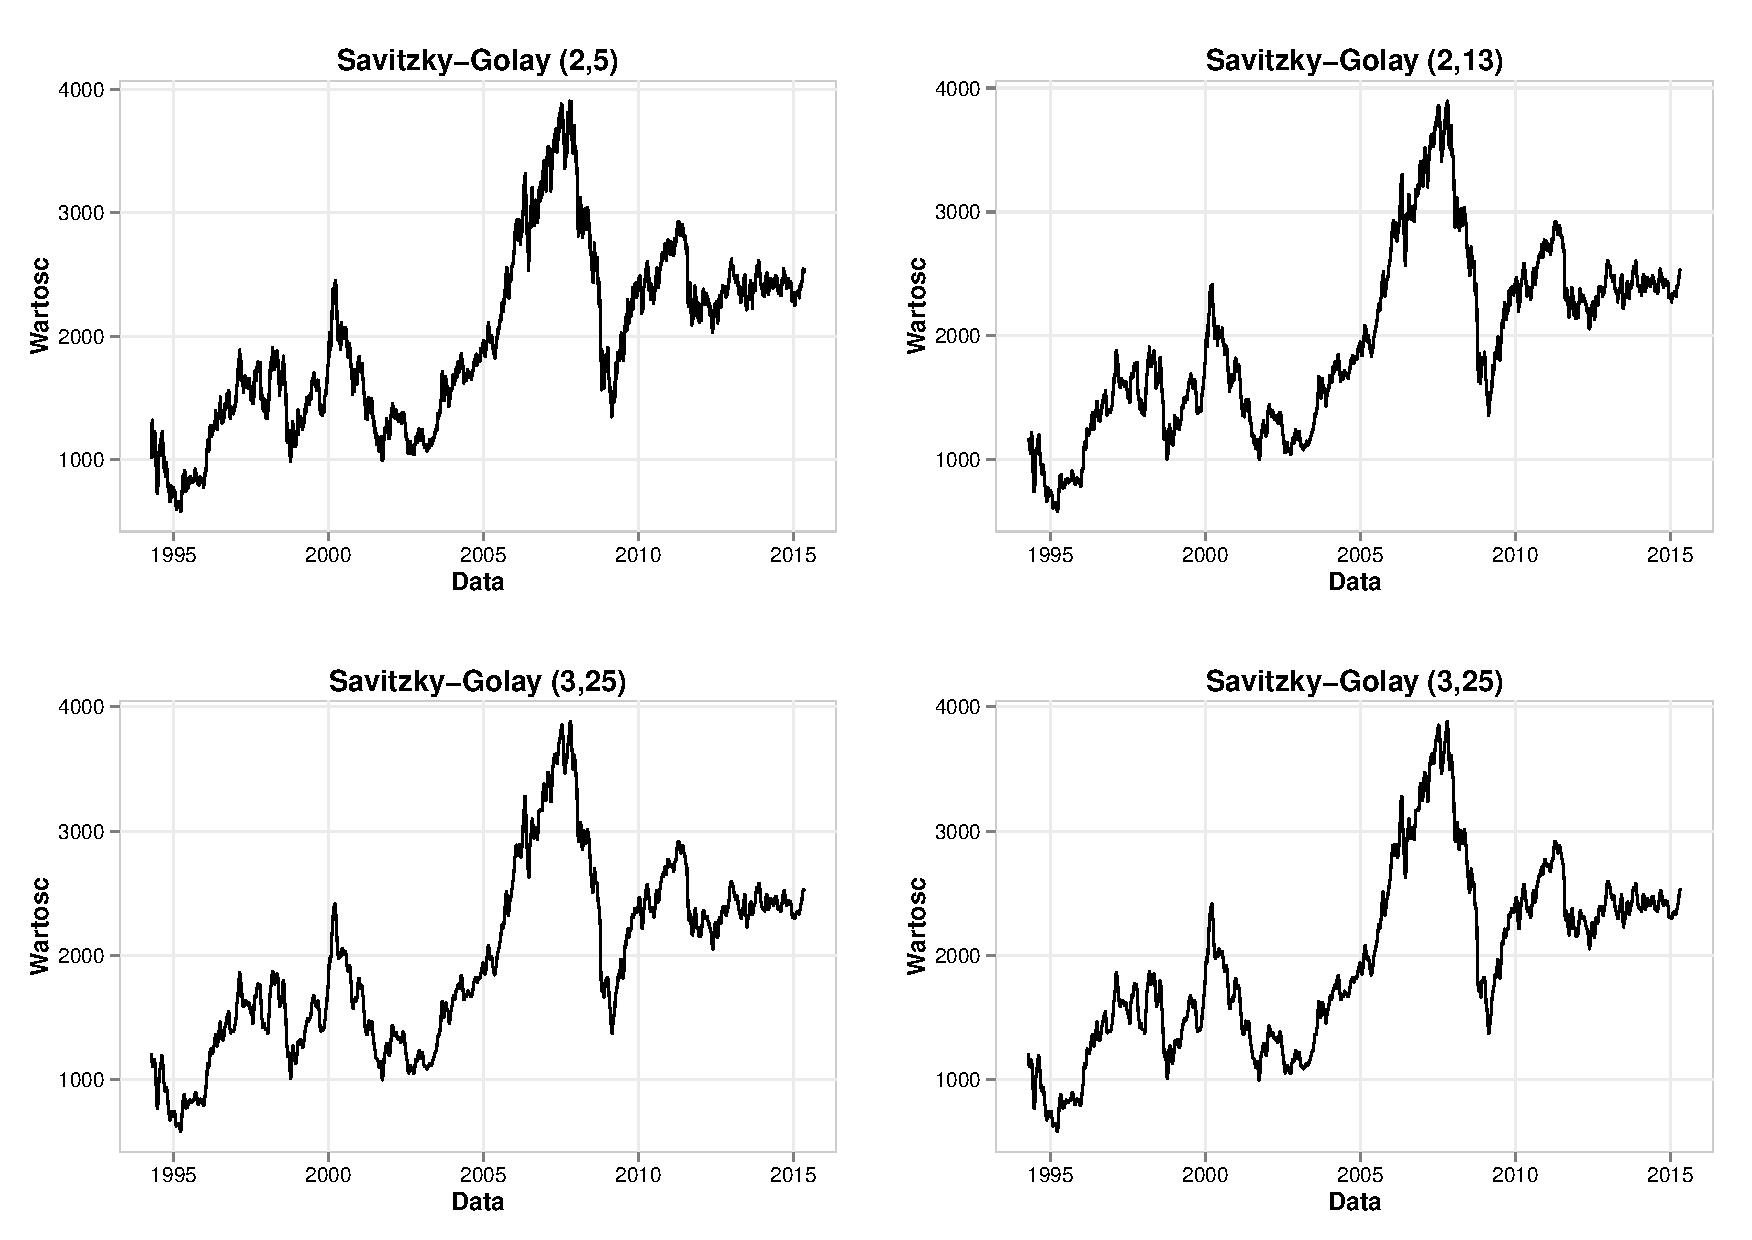
\includegraphics[width=\textwidth]{./rys017}
  \end{subfigure}

  \captionsetup{margin=10pt,font=small,labelfont=bf,width=.8\textwidth}

  \caption[Porównanie zastosowania filtru Savitzky'ego-Golaya dla różnych zestawów parametrów]{Porównanie zastosowania filtru Savitzky'ego-Golaya dla różnych zestawów parametrów. \textit{Źródło:} opracowanie własne}\label{rys017}
\end{figure}

Jako, że przy tak długim szeregu czasowym zależy nam przede wszystkim na ograniczeniu krótkookresowych wahań, ostatni zestaw parametrów (szereg wygładzony za pomocą wielomianu trzeciego stopnia oszacowanego 
za pomocą 25 punktów) wydaje się być najbardziej odpowiedni. Można też dostrzec, że użycie takiej kombinacji nie powoduje zniekształcenia tendencji panującej na rynku w tym okresie (rysunek~\ref{rys002}).

\begin{figure}[H]
  \centering

  \begin{subfigure}[t]{1.00\textwidth}
    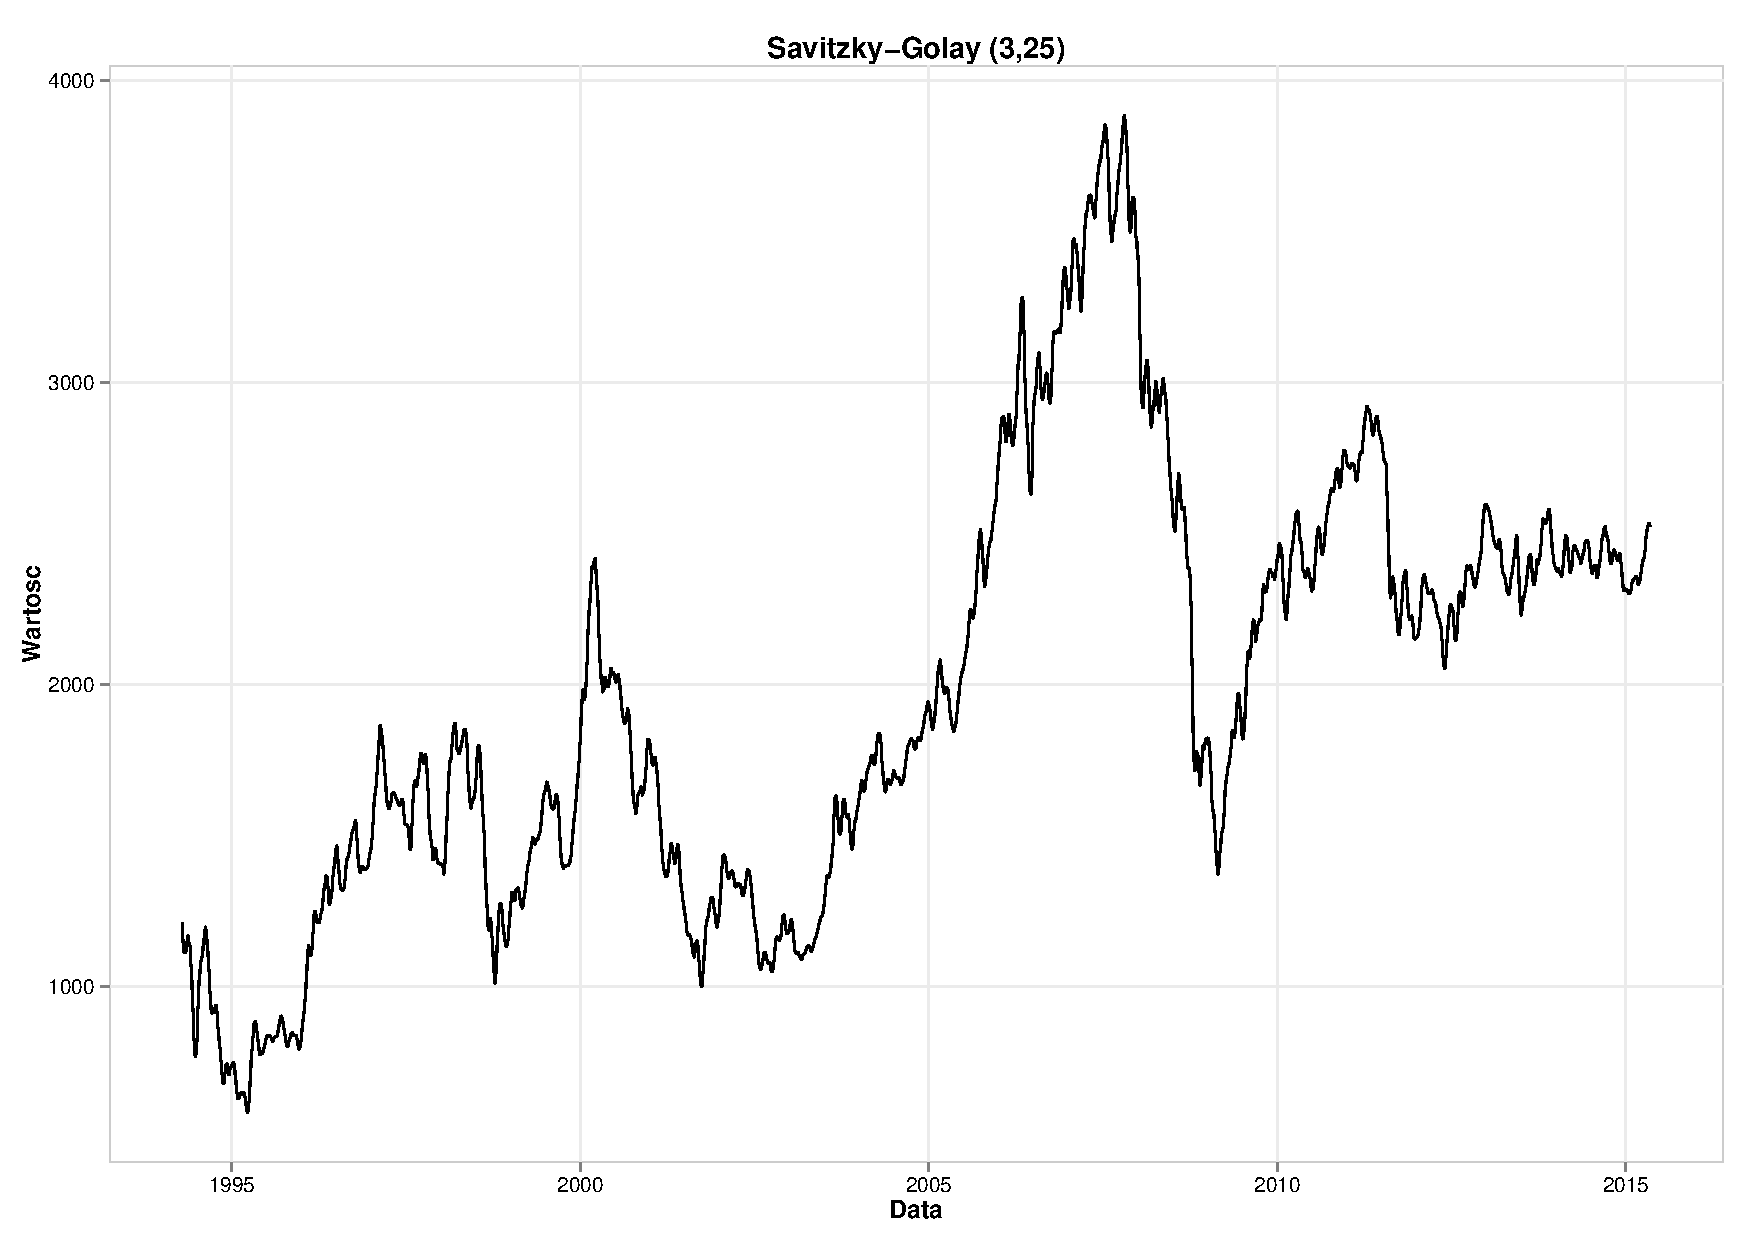
\includegraphics[width=\textwidth]{./rys002}
  \end{subfigure}

  \captionsetup{margin=10pt,font=small,labelfont=bf,width=.8\textwidth}

  \caption[Użyty filtr Savitzky'ego-Golaya]{Zastosowanie filtru Savitzky'ego-Golaya do indeksu WIG20. \textit{Źródło:} opracowanie własne}\label{rys002}
\end{figure}

\subsection{Segmentacja danych}

Kolejny krok algorytmu stanowi segmentacja szeregu. Jako że proponowane wcześniej metody liniowej segmentacji i binarnej segmentacji różnią się znacząco w swoim działaniu, dlatego też ciężko stwierdzić użycie 
którego doprowadzi do lepszych wyników. Z tego względu dalsza część algorytmu przeprowadzana będzie oddzielnie dla obu metod.

Funkcja \(linearSegmentation\) przyjmuje dwa argumenty określające początkową liczbę obserwacji zawartą w każdym segmencie, oraz kąt tolerancji, poniżej którego sąsiednie segmenty są łączone. W naszym przypadku 
wielkość okna ustawiamy na 5 dni, jako że wielkość ta odpowiada długości tygodnia roboczego, kiedy to występuje handel na rynku. Ponadto chcemy wyeliminować tendencje panujące na rynku o krótszym czasie trwania, 
ponieważ są one zazwyczaj o małym znaczeniu i prowadziłyby do nadmiaru informacji. Aby zapobiec powstaniu zbyt małej ilości segmentów spowodowanej dużą tolerancją przy łączeniu sąsiednich okien, drugi argument 
zostaje ustawiony na 0.1\degree . Oznacza to, że w przypadku gdy różnica w kącie nachylenia prostych między segmentami jest większa niż 0.1\degree, wtedy punkt zmiany zostaje odnotowany. W wyniku działania tej funkcji powstało 
877 segmentów.

Następnie w celu połączenia tych okien, których trend jest zbliżony do siebie, stosujemy funkcję \(MergeSimilarTrends\) . Jako próg, poniżej którego dochodzi do zespojenia sąsiadujących elementów, przyjmujemy wartość 
0.5\%. Stosując taki schemat działania, ostatecznie wygenerowane zostaje 700 segmentów. Ich przebieg przedstawia rysunek~\ref{rys004}.

\begin{figure}[H]
  \centering

  \begin{subfigure}[t]{1.00\textwidth}
    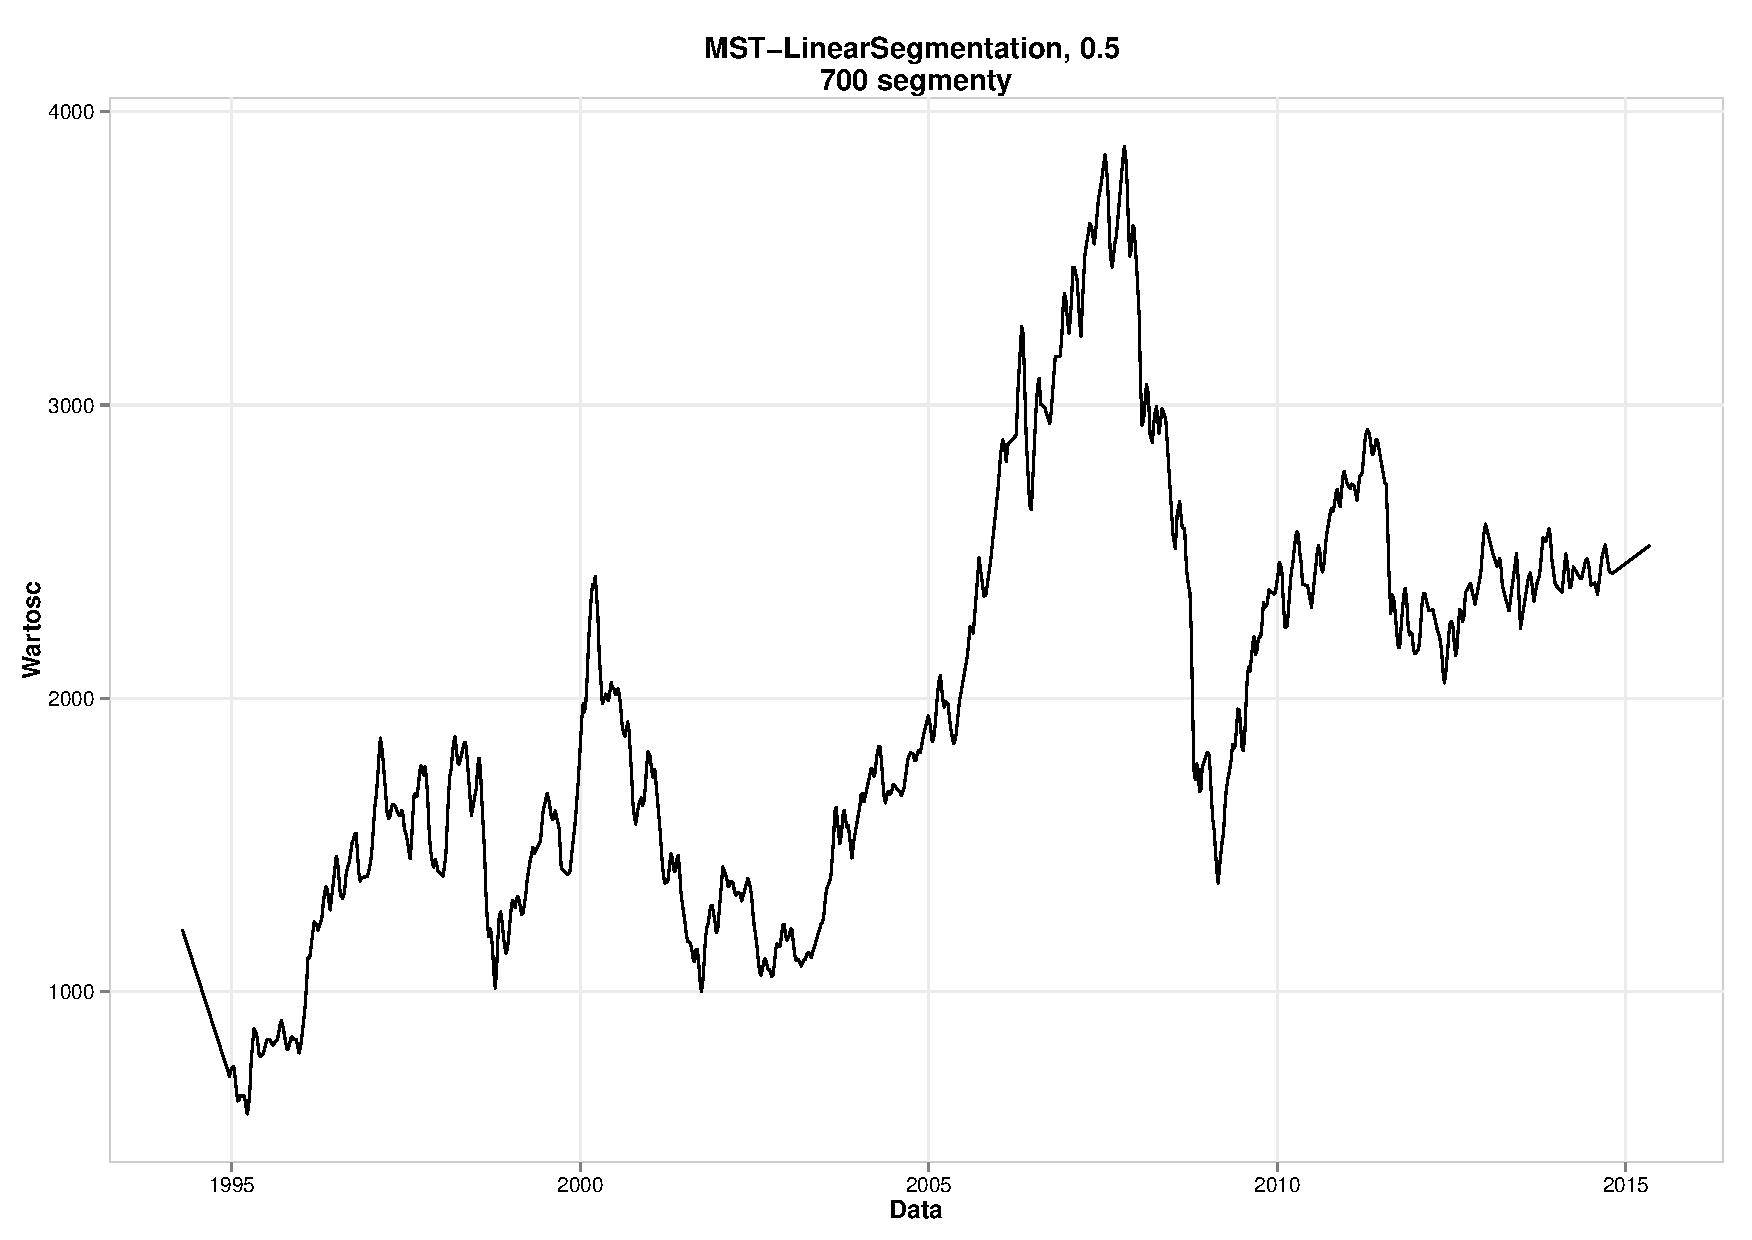
\includegraphics[width=\textwidth]{./rys004}
  \end{subfigure}

  \captionsetup{margin=10pt,font=small,labelfont=bf,width=.8\textwidth}

  \caption[Zastosowanie funkcji linearSegmentation, a następnie MergeSimilarTrends]{Zastosowanie funkcji linearSegmentation, a następnie MergeSimilarTrends do odszumionego szeregu indeksu WIG20. \textit{Źródło:} opracowanie własne}\label{rys004}
\end{figure}

Drugim podejściem jest zastosowanie funkcji \(cpt.mean\). Jeden z parametrów tej funkcji każe określić, czy dane użyte do segmentacji mają rozkład normalny w celu doboru odpowiedniego testu statystycznego.

Aby tego dokonać, użyty zostanie test Kołmogorowa-Smirnova. Jest to test nieparametryczny, pozwalający na badanie podobieństwa rozkładu danej zmiennej z innym rozkładem. W naszym 
przypadku hipoteza zerowa zakłada, że rozkład wygładzonych obserwacji indeksu WIG20 jest zbliżony do normalnego.

Histogramy odfiltrowanych obserwacji oraz ich pierwszych różnic przedstawia rysunek~\ref{rys015} oraz rysunek~\ref{rys016}. Wartości p-value dla przeprowadzonych testów prezentuje tabela~\ref{tab001}.

\begin{figure}[H]
  \centering

  \begin{subfigure}[t]{1.00\textwidth}
    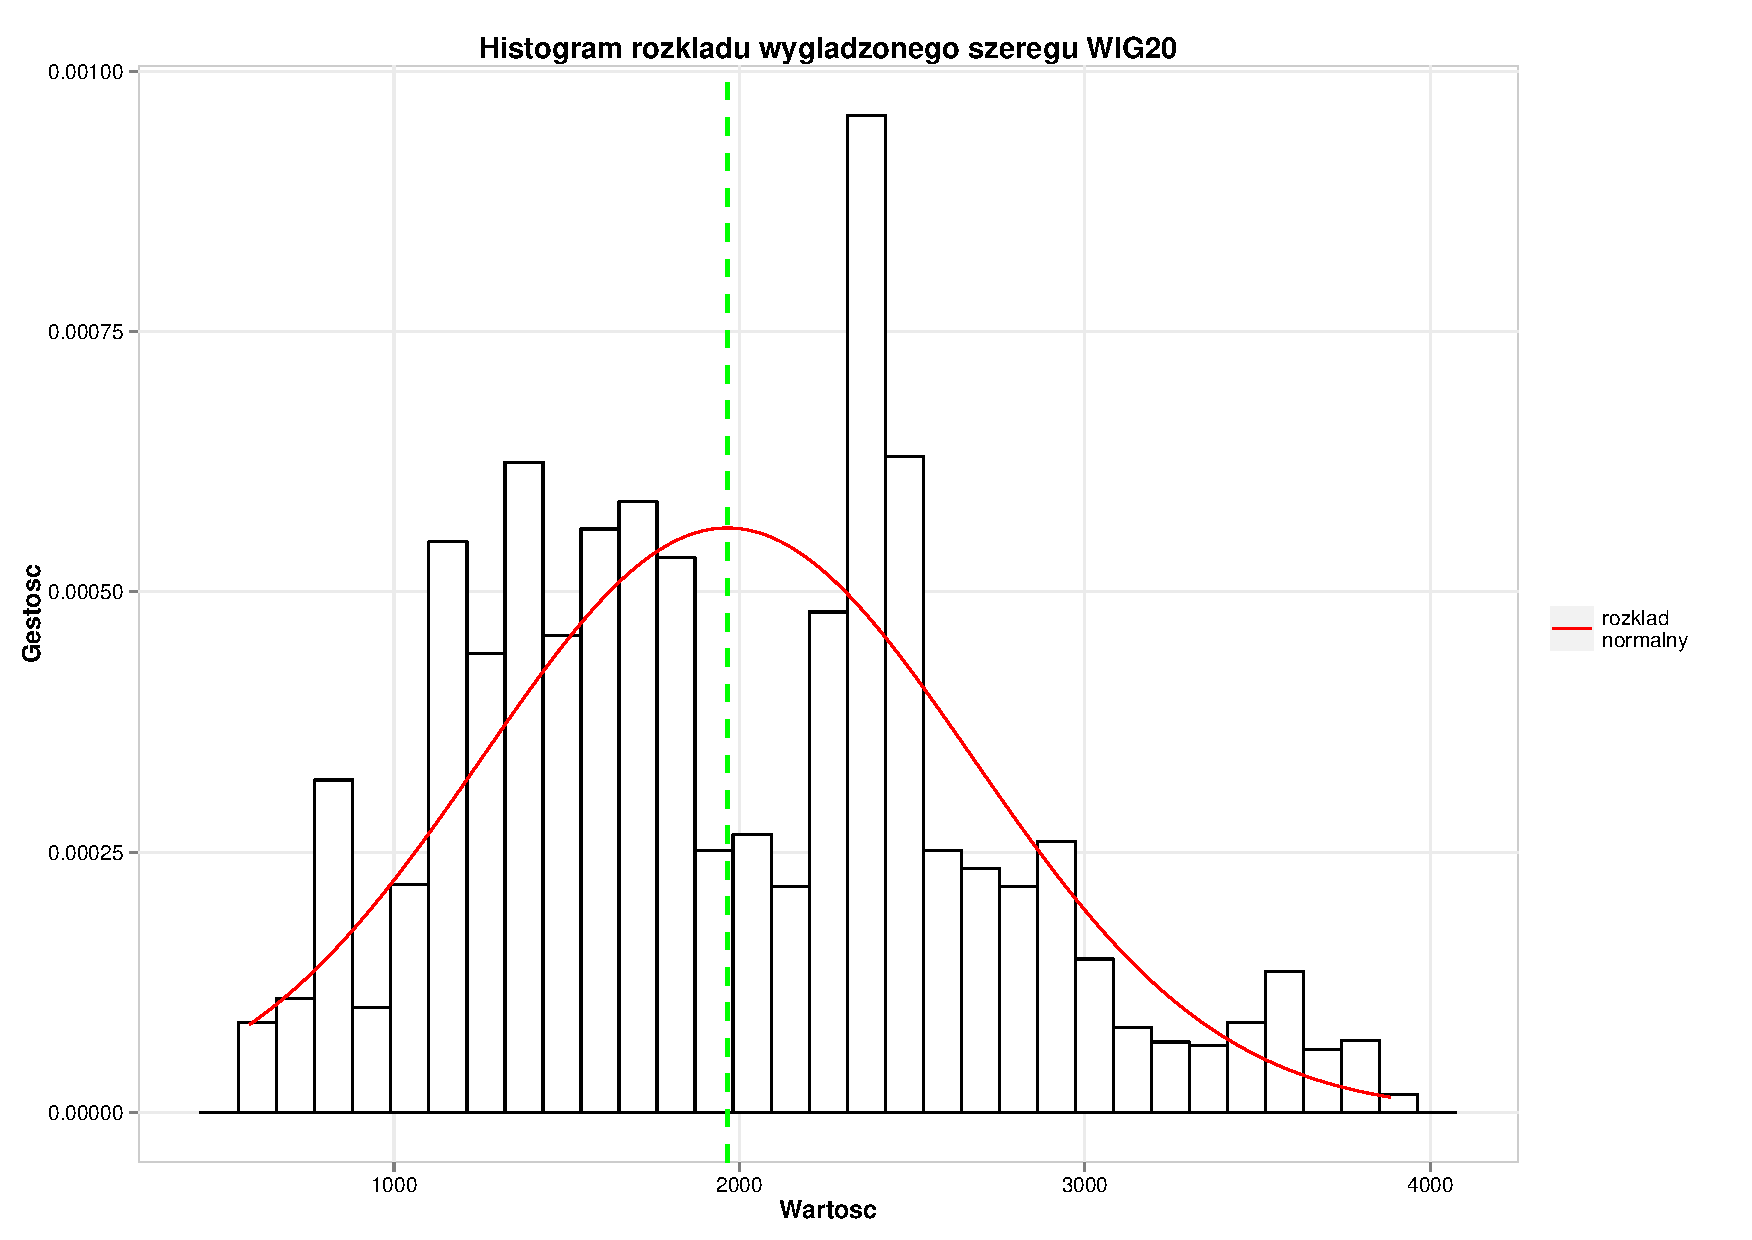
\includegraphics[width=\textwidth]{./rys015}
  \end{subfigure}

  \captionsetup{margin=10pt,font=small,labelfont=bf,width=.8\textwidth}

  \caption[Histogram rozkladu wygladzonego szeregu WIG20]{Histogram rozkladu wygladzonego szeregu WIG20. \textit{Źródło:} opracowanie własne}\label{rys015}
\end{figure}

\begin{figure}[H]
  \centering

  \begin{subfigure}[t]{1.00\textwidth}
    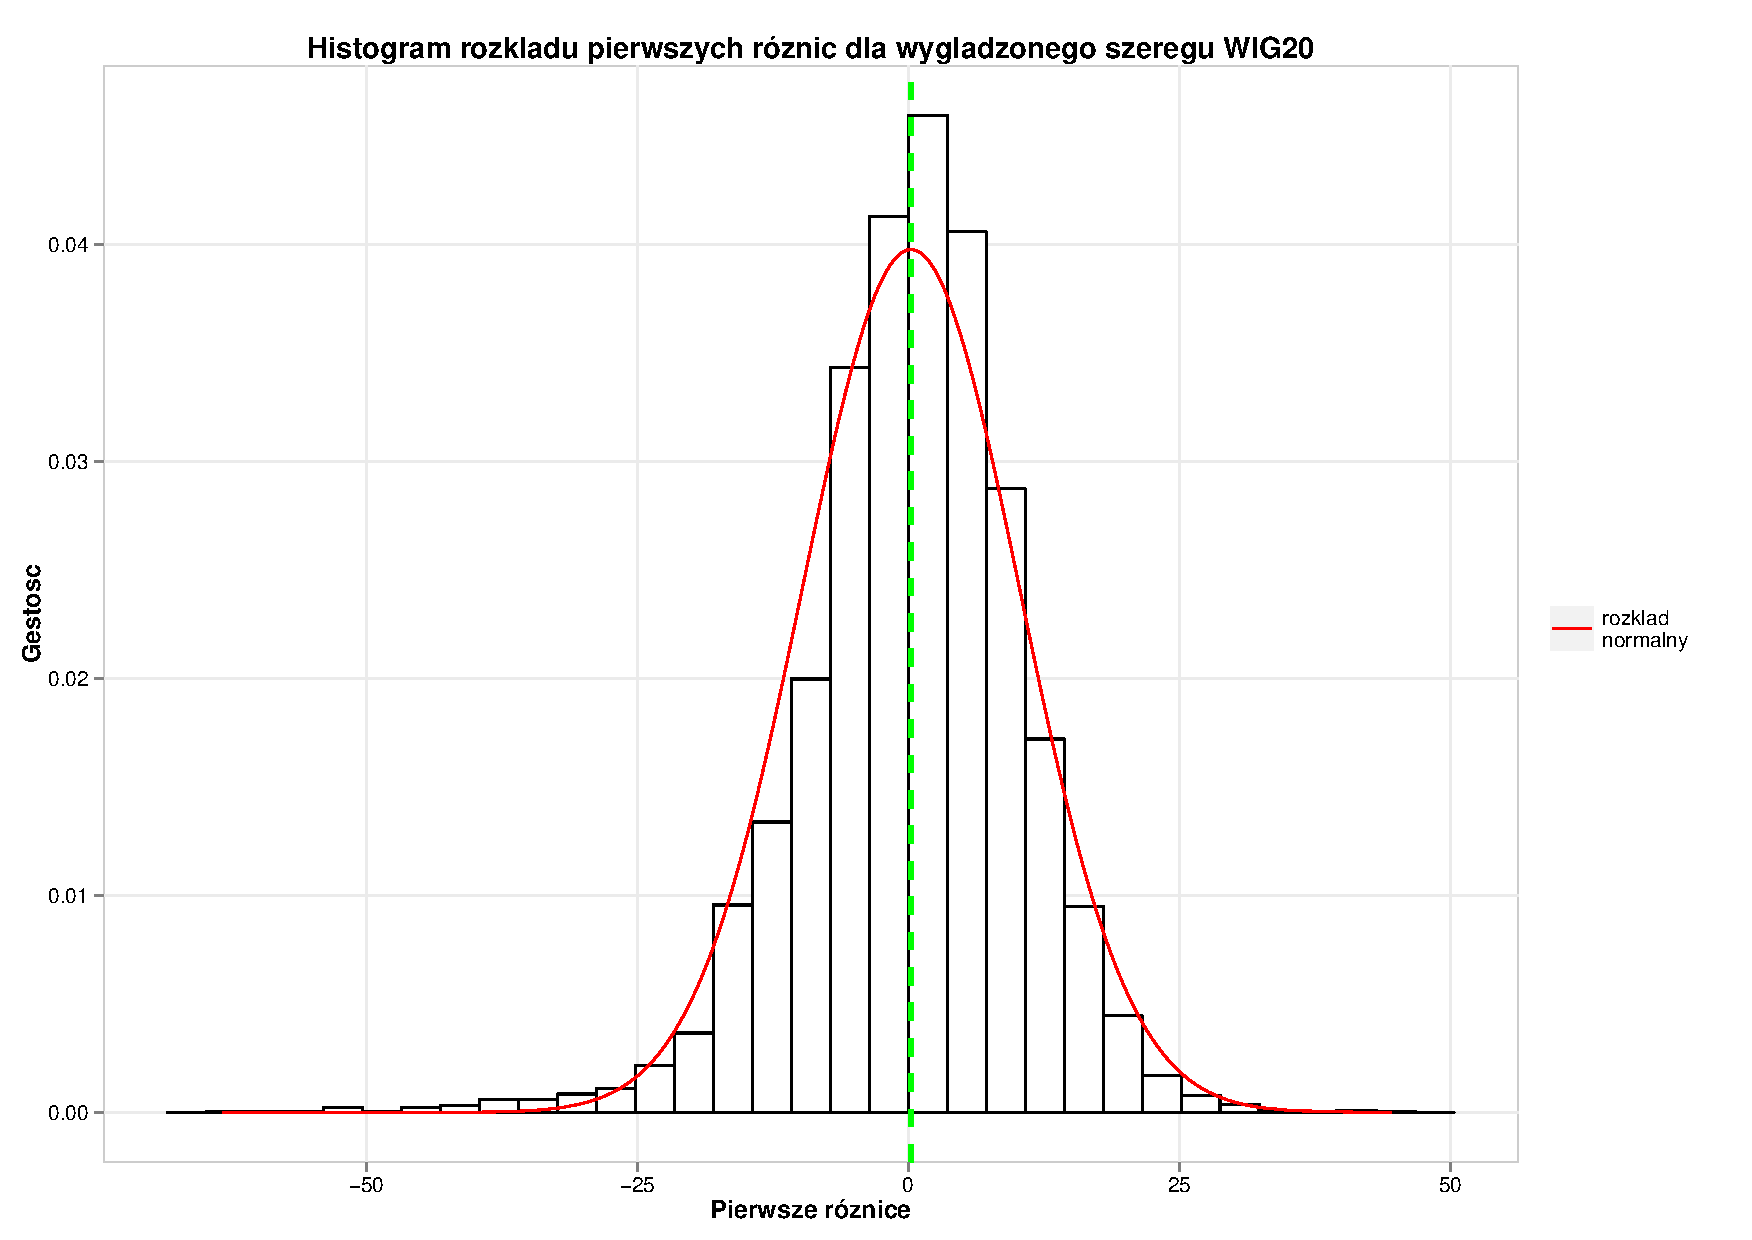
\includegraphics[width=\textwidth]{./rys016}
  \end{subfigure}

  \captionsetup{margin=10pt,font=small,labelfont=bf,width=.8\textwidth}

  \caption[Histogram rozkladu pierwszych różnic wygladzonego szeregu WIG20]{Histogram rozkladu pierwszych różnic wygladzonego szeregu WIG20. \textit{Źródło:} opracowanie własne}\label{rys016}
\end{figure}

\begin{table}[H] \centering
\caption{Wartości p-value dla testu Kołmogorowa-Smirnova. \textit{Źródło:} opracowanie własne}
\label{tab001}
\begin{tabular}{lrr}
\(data\)    & \(wygladzone\)       & \(diff(wygladzone)\)   \\ \hline
D       & 1                & 0.4221            \\
p-value & \textless2.2e-16 & \textless2.2e-16 
\end{tabular}
\end{table}


Na podstawie wartości p-value odrzucamy hipotezę zerową i stwierdzamy, iż nasza zmienna posiada rozkład różny od normalnego. Dlatego też argument \(test.stat\) określamy jako \(CUSUM\). Jako funkcję 
kary, chroniącą przed zbytnim dopasowaniem, przyjmujemy kryterium informacyjne Hannana-Quinna.

Po zaaplikowaniu tej funkcji otrzymujemy 1186 segmenty. Nastepnie, analogicznie jak w poprzedniej metodzie, stosujemy funkcję \(MergeSimilarTrends\), przyjmując próg również w wysokości 0.5\%. Ostatecznie 
szereg zostaje podzielony na 453 segmenty. Rysunek~\ref{rys003} przedstawia końcowy efekt użycia funkcji \(cpt.mean\) oraz \(MergeSimilarTrends\), natomiast rysunek~\ref{rys005} pokazuje porównanie 
pierwotnego szeregu czasowego, szeregu po użyciu filtru oraż po użyciu liniowej i binarnej segmentacji.

\begin{figure}[H]
  \centering

  \begin{subfigure}[t]{1.00\textwidth}
    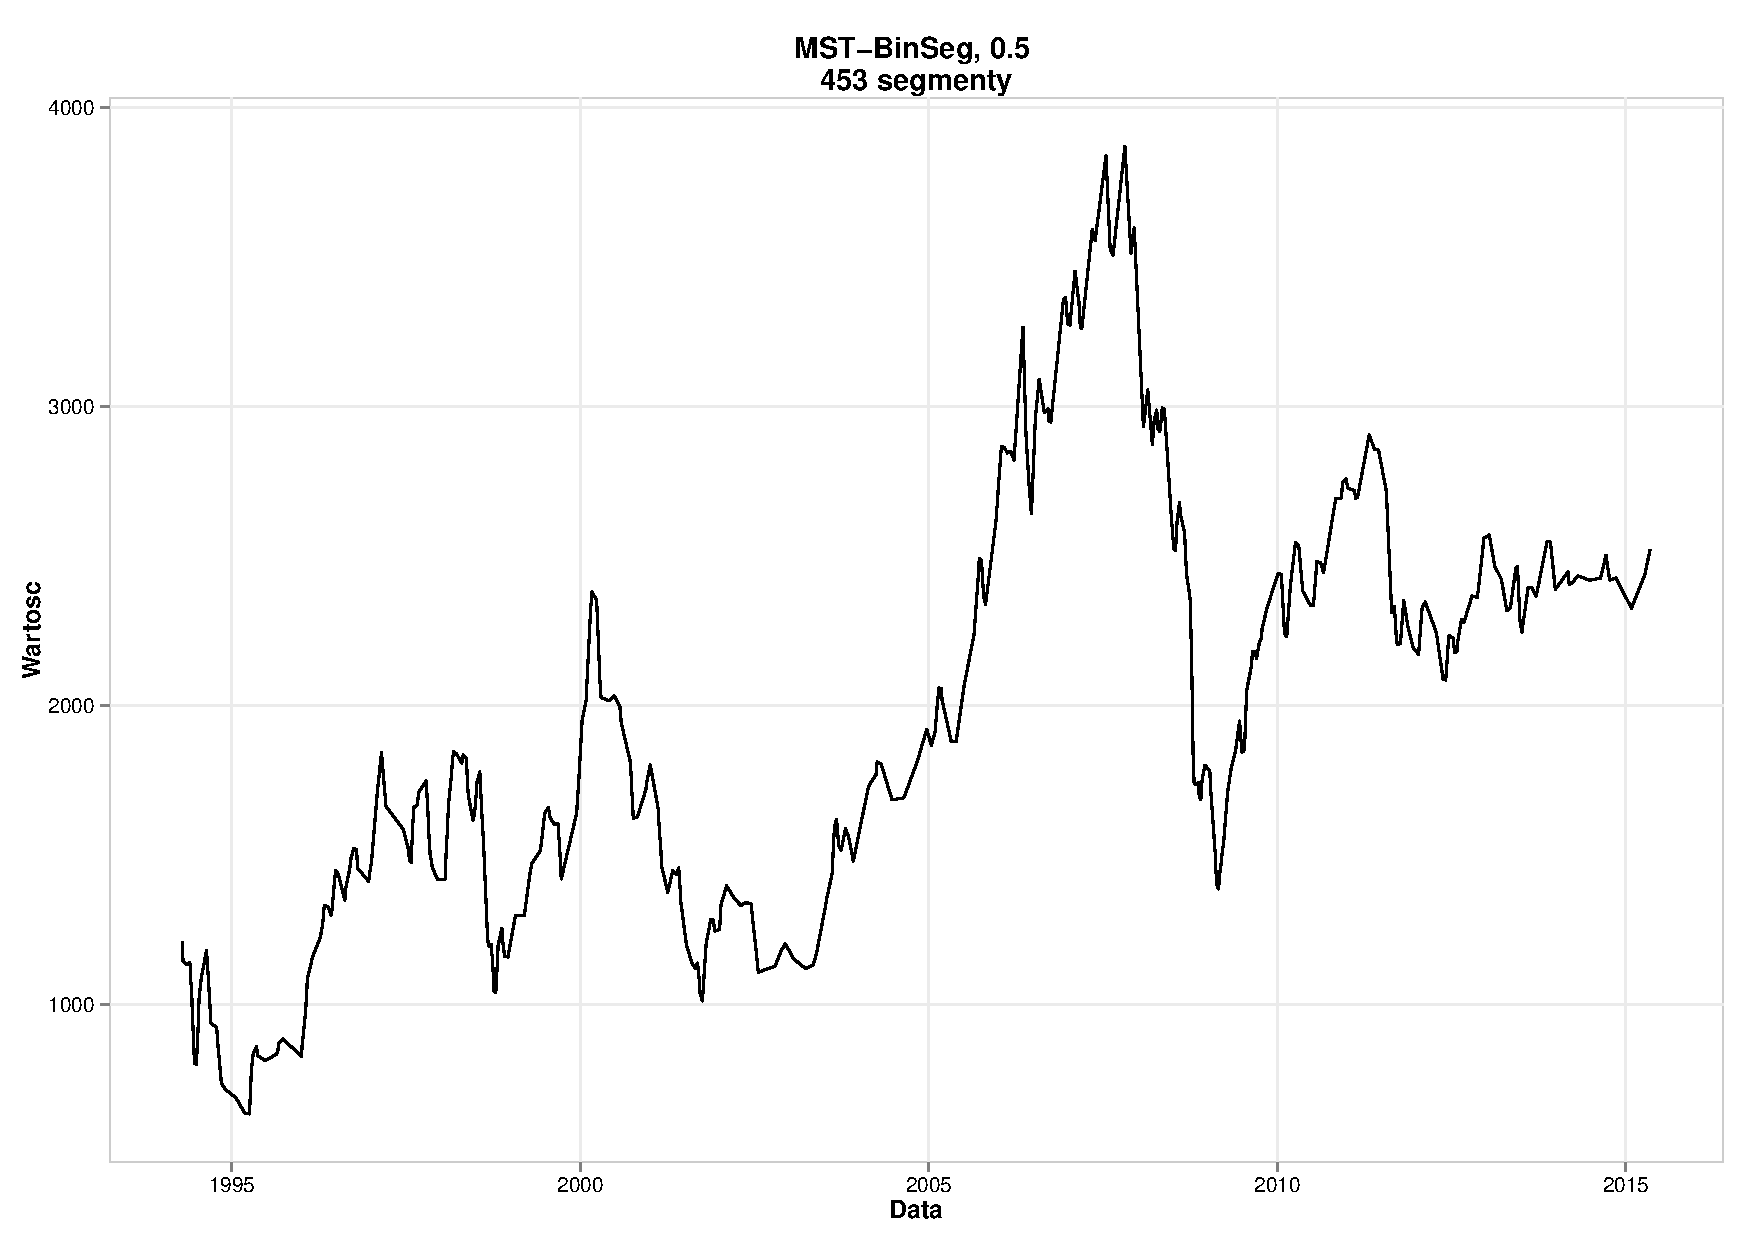
\includegraphics[width=\textwidth]{./rys003}
  \end{subfigure}

  \captionsetup{margin=10pt,font=small,labelfont=bf,width=.8\textwidth}

  \caption[Zastosowanie funkcji cpt.mean, a następnie MergeSimilarTrends]{Zastosowanie funkcji cpt.mean, a następnie MergeSimilarTrends do odszumionego szeregu indeksu WIG20. \textit{Źródło:} opracowanie własne}\label{rys003}
\end{figure}

\begin{figure}[H]
  \centering

  \begin{subfigure}[t]{1.00\textwidth}
    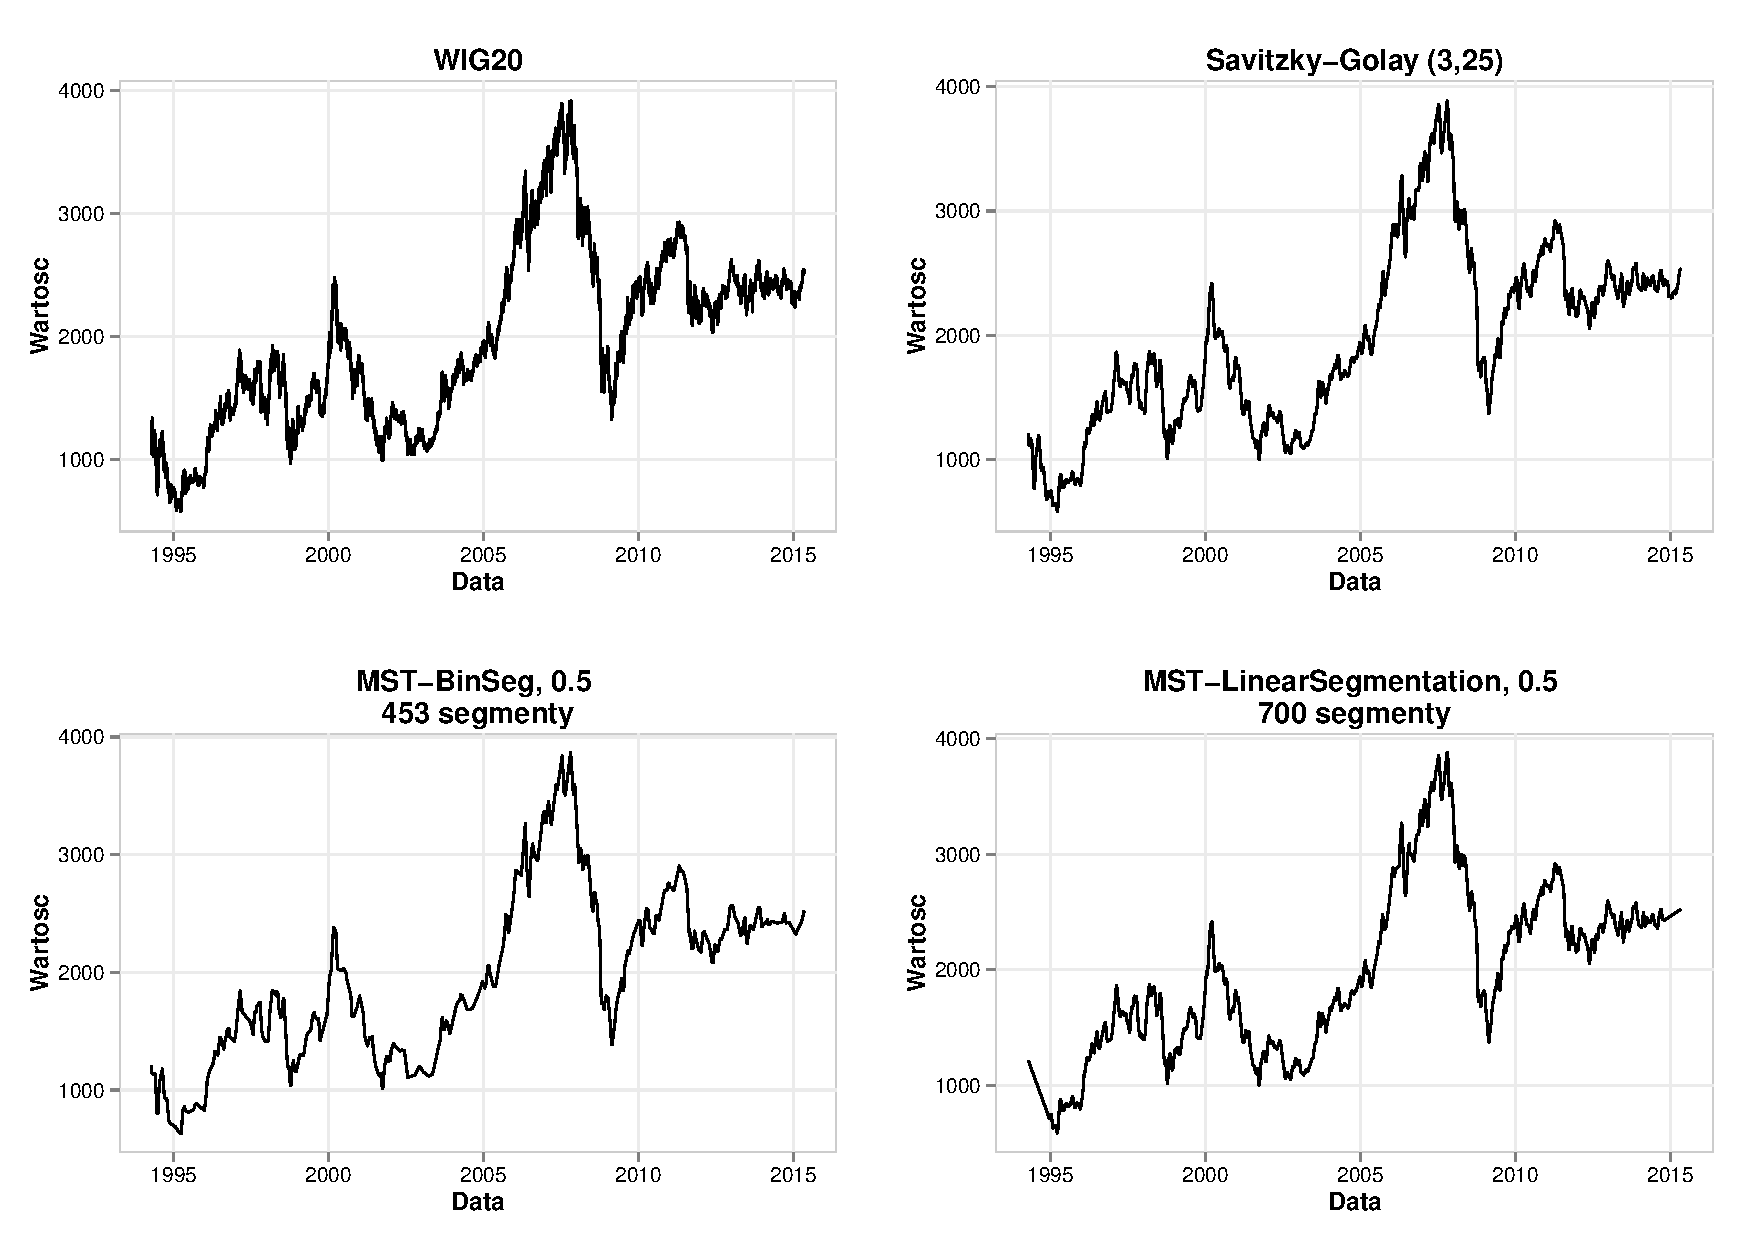
\includegraphics[width=\textwidth]{./rys005}
  \end{subfigure}

  \captionsetup{margin=10pt,font=small,labelfont=bf,width=.8\textwidth}

  \caption[Porównanie pierwotnego, odszumionego i posegmentowanego szeregu WIG20]{Porównanie pierwotnego, odszumionego i posegmentowanego szeregu WIG20. \textit{Źródło:} opracowanie własne}\label{rys005}
\end{figure}

\subsection{Budowa słownika}

Przyszedł czas na konwersję otrzymanych segmentów na łatwe w interpretacji i wnioskowaniu klasy. Aby tego dokonać, przyjrzyjmy się bliżej podstawowym statystykom opisowym 
dotyczącym trendu oraz czasu trwania segmentów dla obu metod (tabela~\ref{tab002},\ref{tab003}).

 \begin{table}[H]
\caption{Statystyki opisowe dotyczące trendu w segmentach. \textit{Źródło:} opracowanie własne}
\label{tab002} 
\begin{tabular}{lrrrrrr}
Metoda   &  Min. &  1st Qu.  &  Median  &  Mean   &  3rd Qu. & Max. \\ \hline
LinearSegmentation &-39.9000 &  -1.8170  &  0.1180  &  0.1874  &  2.1670  & 14.9300 \\
BinarySegmentation & -19.92000 & -2.03900 & -0.09549 &  0.28410 &  2.49500 & 18.51000 
 \end{tabular}
 \end{table}


 \begin{table}[H]
\caption{Statystyki opisowe dotyczące czasu trwania poszczególnych segmentów. \textit{Źródło:} opracowanie własne}
\label{tab003}
 \begin{tabular}{lrrrrrr}
Metoda   &  Min. &  1st Qu.  &  Median  &  Mean   &  3rd Qu. & Max. \\ \hline
LinearSegmentation &   0.000  & 5.000 &  5.000 &  7.477  & 8.000 & 131.000 \\
BinarySegmentation &  0.00  &  3.00 &   8.00 &  11.55 &  16.00 &  66.00 
 \end{tabular}
 \end{table}

Można zauważyć, iż segmenty utworzone za pomocą funkcji \(linear Segmentation\) charakteryzują się bardziej ekstremalnymi wartościami jeśli chodzi o trend. Zastosowanie binarnej 
segmentacji prowadzi natomiast do powstania okien o węższym zakresie trendu, jednakże wartości pierwszego i trzeciego kwantyla sugerują, że więcej obserwacji znajduje się w ogonach 
rozkładu. Ujemna mediana wskazuje także na większą liczbe segmentów z trendem spadkowym. Jeśli chodzi o czas trwania poszczególnych okien, mediana i średnia w przypadku segmentacji 
liniowej wskazują na dużą liczbę fragmentów o długości 5 dni, czyli tych przyjętych w funkcji jako początkową szerokość każdego okna. Pomimo informacji uzyskanych za pomocą 
statystyk opisowych, chcąc dokonać podziału tych dwóch zmiennych na określoną ilość klas, potrzebowalibyśmy przeanalizować jaki rozkład mają te zmienne. W tym celu posłużymy się 
histogramami czasu trwania i trendu(wykres~\ref{rys018},\ref{rys019}).

\begin{figure}[H]
  \centering
  \begin{subfigure}[t]{0.45\textwidth}
    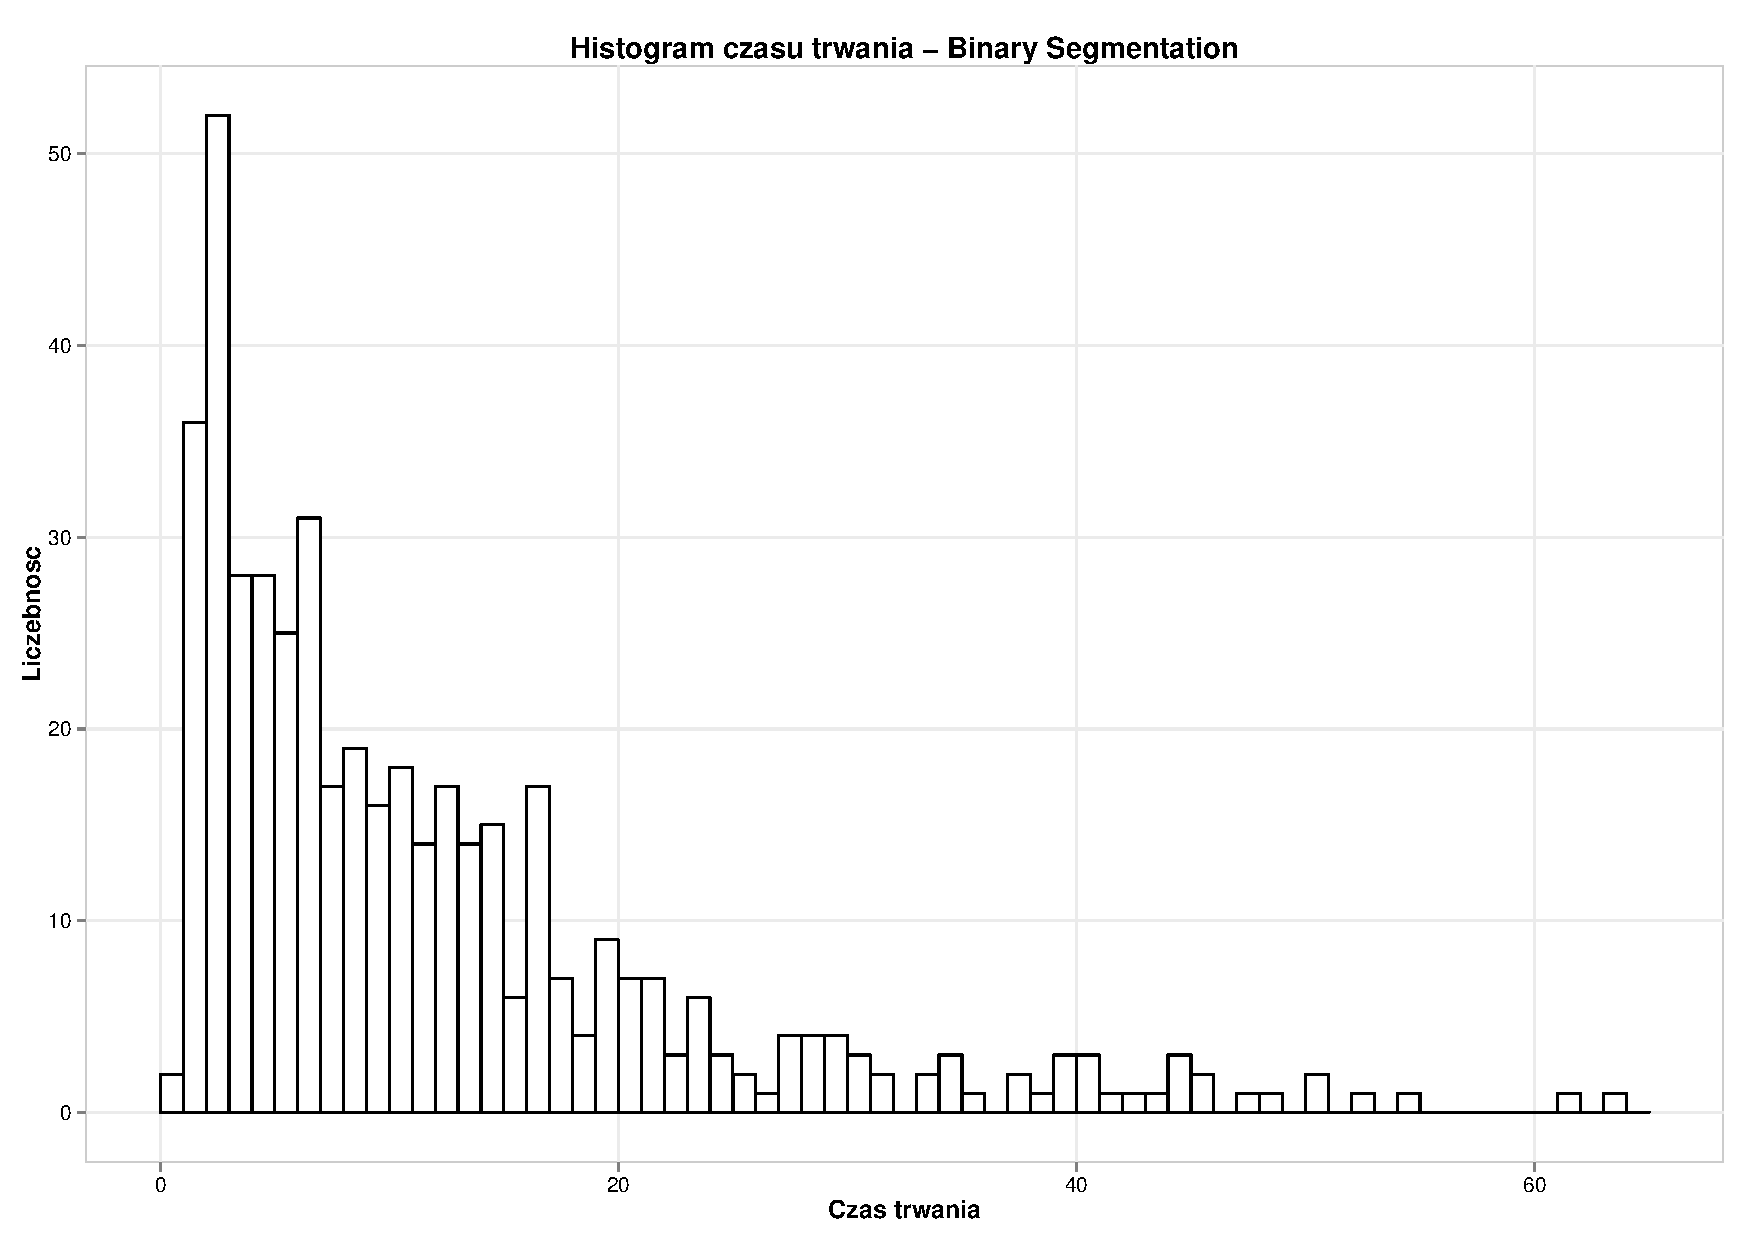
\includegraphics[width=\textwidth]{./rys006}
    \caption{Binary Segmentation}
    \label{xxxa}
  \end{subfigure}
  \hfill
  \begin{subfigure}[t]{0.45\textwidth}
    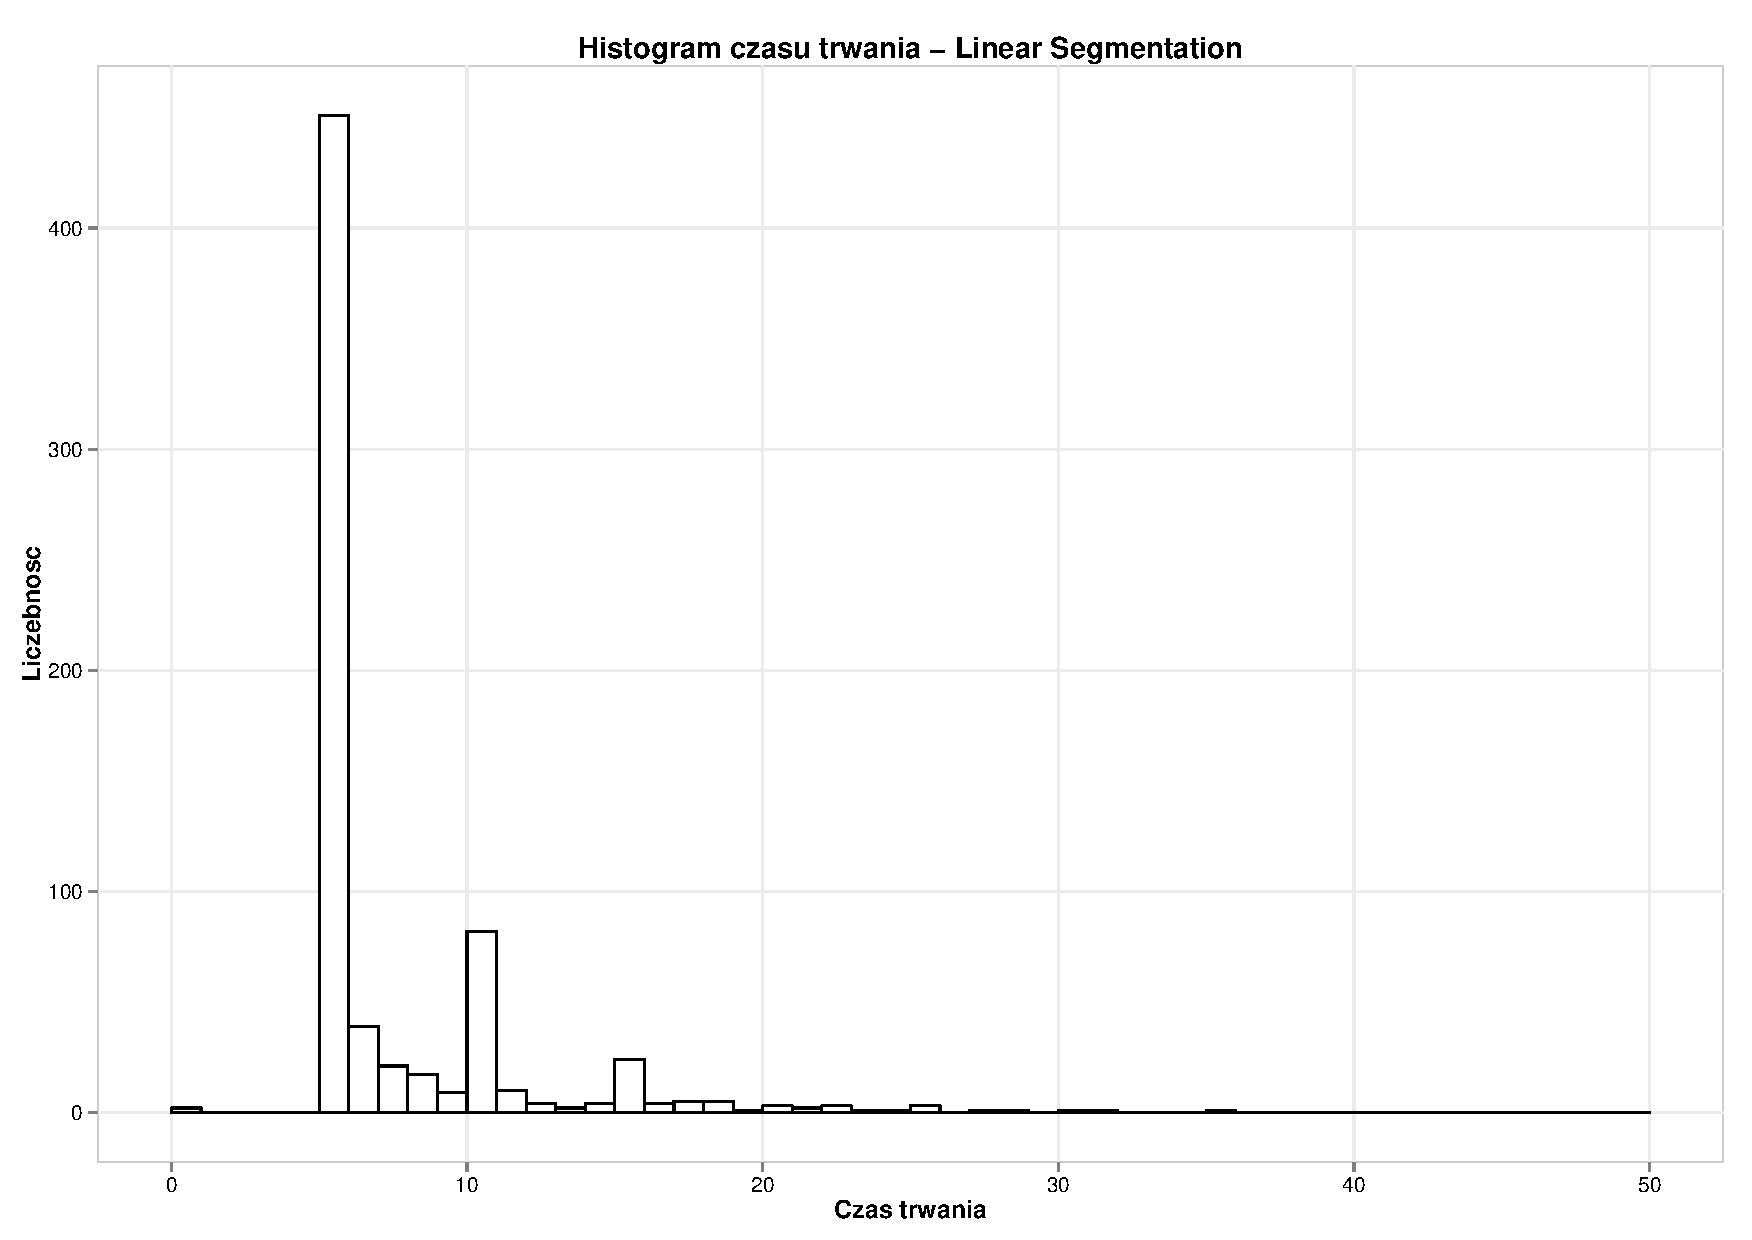
\includegraphics[width=\textwidth]{./rys007}
    \caption{Linear Segmentation}
    \label{xxxb}
  \end{subfigure}
  \captionsetup{margin=10pt,font=small,labelfont=bf,width=.8\textwidth}
  \caption[Histogram czasu trwania- segmentacja liniowa oraz binarna]{Histogram czasu trwania poszczególnych segmentów dla odpowiednich metod. \textit{Źródło:} opracowanie własne}\label{rys018}
\end{figure}


\begin{figure}[H]
  \centering
  \begin{subfigure}[t]{0.45\textwidth}
    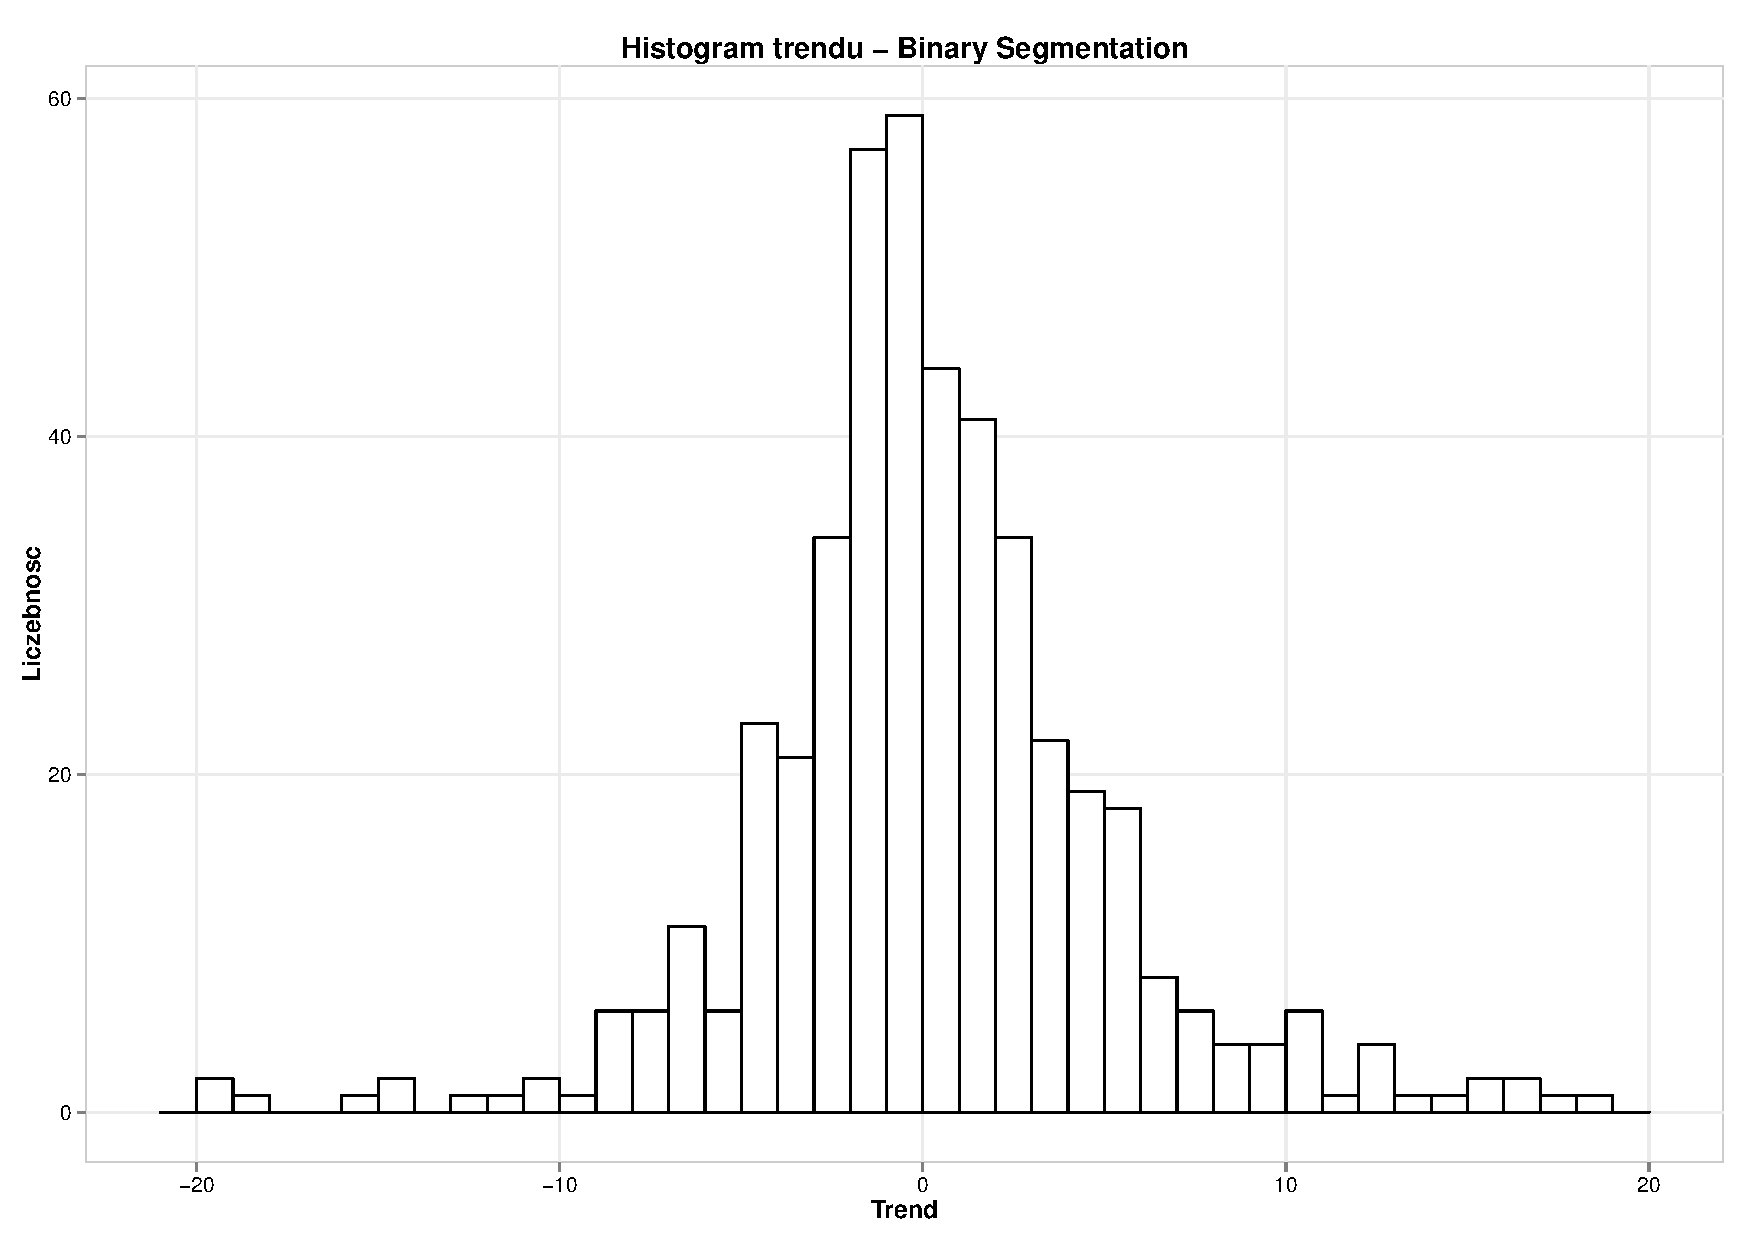
\includegraphics[width=\textwidth]{./rys008}
    \caption{Binary Segmentation}
    \label{xxxc}
  \end{subfigure}
  \hfill
  \begin{subfigure}[t]{0.45\textwidth}
    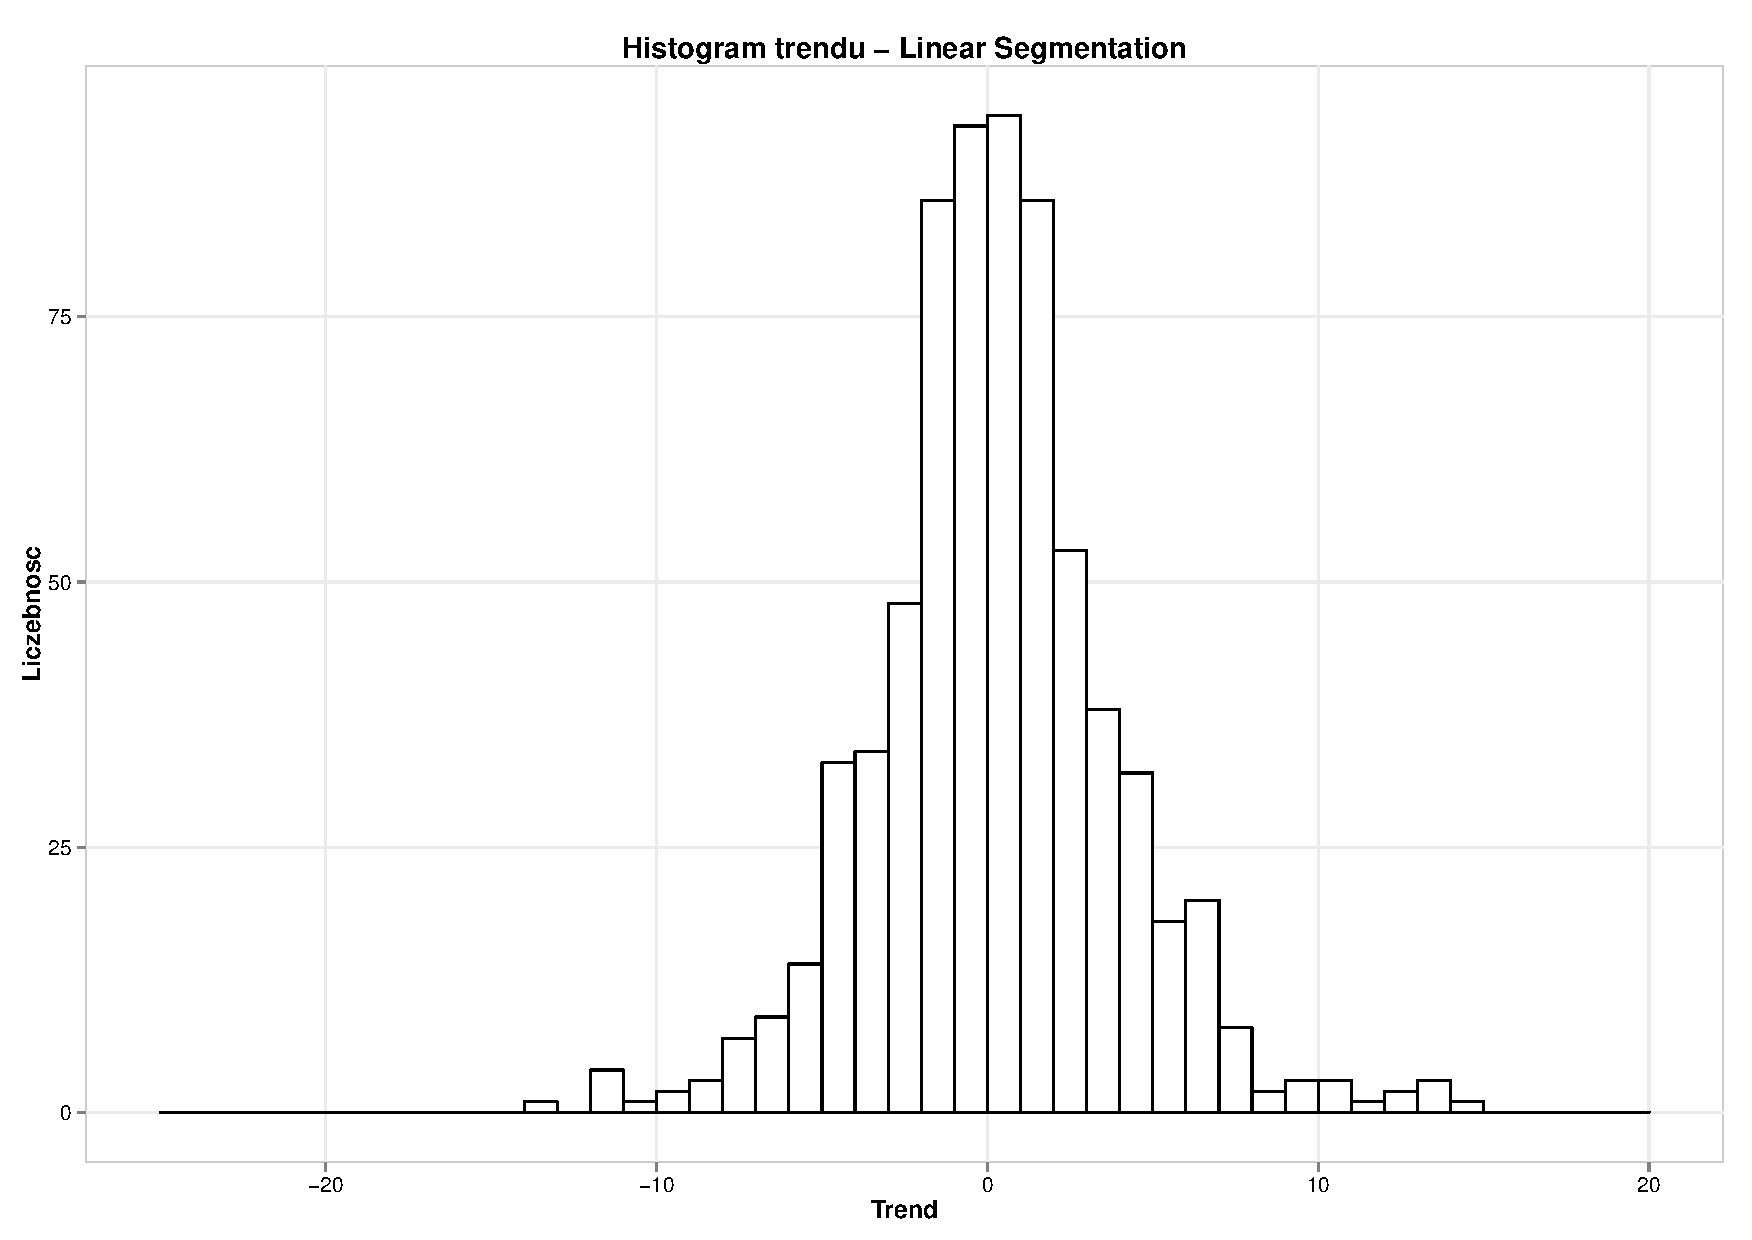
\includegraphics[width=\textwidth]{./rys009}
    \caption{Linear Segmentation}
    \label{xxxd}
  \end{subfigure}
  \captionsetup{margin=10pt,font=small,labelfont=bf,width=.8\textwidth}
  \caption[Histogram trendów panujących w segmentach dla segmentacji liniowej oraz binarnej]{Histogram trendów panujących w segmentach dla poszczególnych metod. \textit{Źródło:} opracowanie własne}\label{rys019}
\end{figure}

Jak widać, jeśli chodzi o czas trwania poszczególnych okien, segmentacja binarna zdaje się dawać bardziej rozłożone wyniki, podczas gdy użycie segmentacji liniowej, jak już wcześniej 
zostało zauważone, powoduje że znaczna większość fragmentów pozostaje długości podanej początkowo do funkcji. W przypadku trendu widać, że oba rozkłady są zbliżone do siebie, najczęstszą 
grupą segmentów są te o trendzie oscylującym koło zera. Widoczne jest jednak większe skupienie segmentów z tendencją spadkową dla \(Binary Segmentation\).

Posiadając takie dane możliwe jest wnioskowanie na temat stworzenia odpowiednich elementów do słownika. Przykładowo czas trwania okien utworzonych za pomocą funkcji \(cpt.mean\) możnaby 
podzielić na 3 przedziały: $\left<0, 5 \right)$, $\left<5, 15 \right)$, $\left<15, \infty \right)$ i sklasyfikować je za pomocą symboli: \(S\) (krótki czasowo segment), \(M\) (segment o średniej długości), \(L\) (segment długoterminowy). Powyższe 
uporządkowanie doprowadziłoby do następującej alokacji obserwacji w tych klasach: 37.75\%, 36.87\%, 25.38\%. Analogicznie podziału możnaby dokonać dla trendu wydzielając 5 klas: \(VN\) (trendy o charakterystyce skrajnie 
spadkowej dla przedziału $\left(-\infty, -4\right>$)  , \(N\) (trendy spadkowe dla przedziału  $\left(-4, -1\right>$), \(C\) (trendy horyzontalne dla przedziału  $\left(-1, 1\right>$), \(P\) (trendy wzrostowe dla przedziału  
$\left(1, 5\right>$) oraz \(VP\) (trendy o charakterystyce wyraźnie wzrostowej dla przedziału  $\left(5, \infty \right>$). Taki podział spowodowałby, że kolejno w każdej z tych klas znalazłoby się 13.9\%, 24.72\%, 
22.74\%, 25.6\%, 13.04\% obserwacji.

W wyniku powyższej reprezentacji symbolicznej utworzonych zostałoby 15 klas opisujących poszczególne okna  (np.: klasa \(VN\_L\) oznaczałaby segment o długim przedziale czasowym, w którym 
występował trend spadkowy). Takie postępowanie sprawia jednak kilka problemów, z których głównym jest subiektywność. Dotyczy ona zarówno doboru liczby klas, jak i wartości 
granicznych. Tworząc bowiem wyżej wymienione klasy, starałem się dobrać parametry tak, aby alokacja obserwacji w każdej z grup była jak najbardziej zrównoważona. Jednakże takie postepowanie może okazać się 
błędne, ponieważ mogą istnieć w zbiorze pewne mniej liczne grupy o właściwościach odbiegających od pozostałych. Dlatego też właściwszym wydaje się zastosowanie metody k-średnich, która wyróżnia zbiory 
składające się z obserwacji podobnych do siebie, a jej jedynym parametrem jest liczba grup. Aby właściwie dobrać tą zmienną przyjrzyjmy się wykresom rozrzutu trendu i czasu trwania dla obu metod (wykres~\ref{rys010}, 
\ref{rys011}).

\begin{figure}[H]
  \centering

  \begin{subfigure}[t]{1.00\textwidth}
    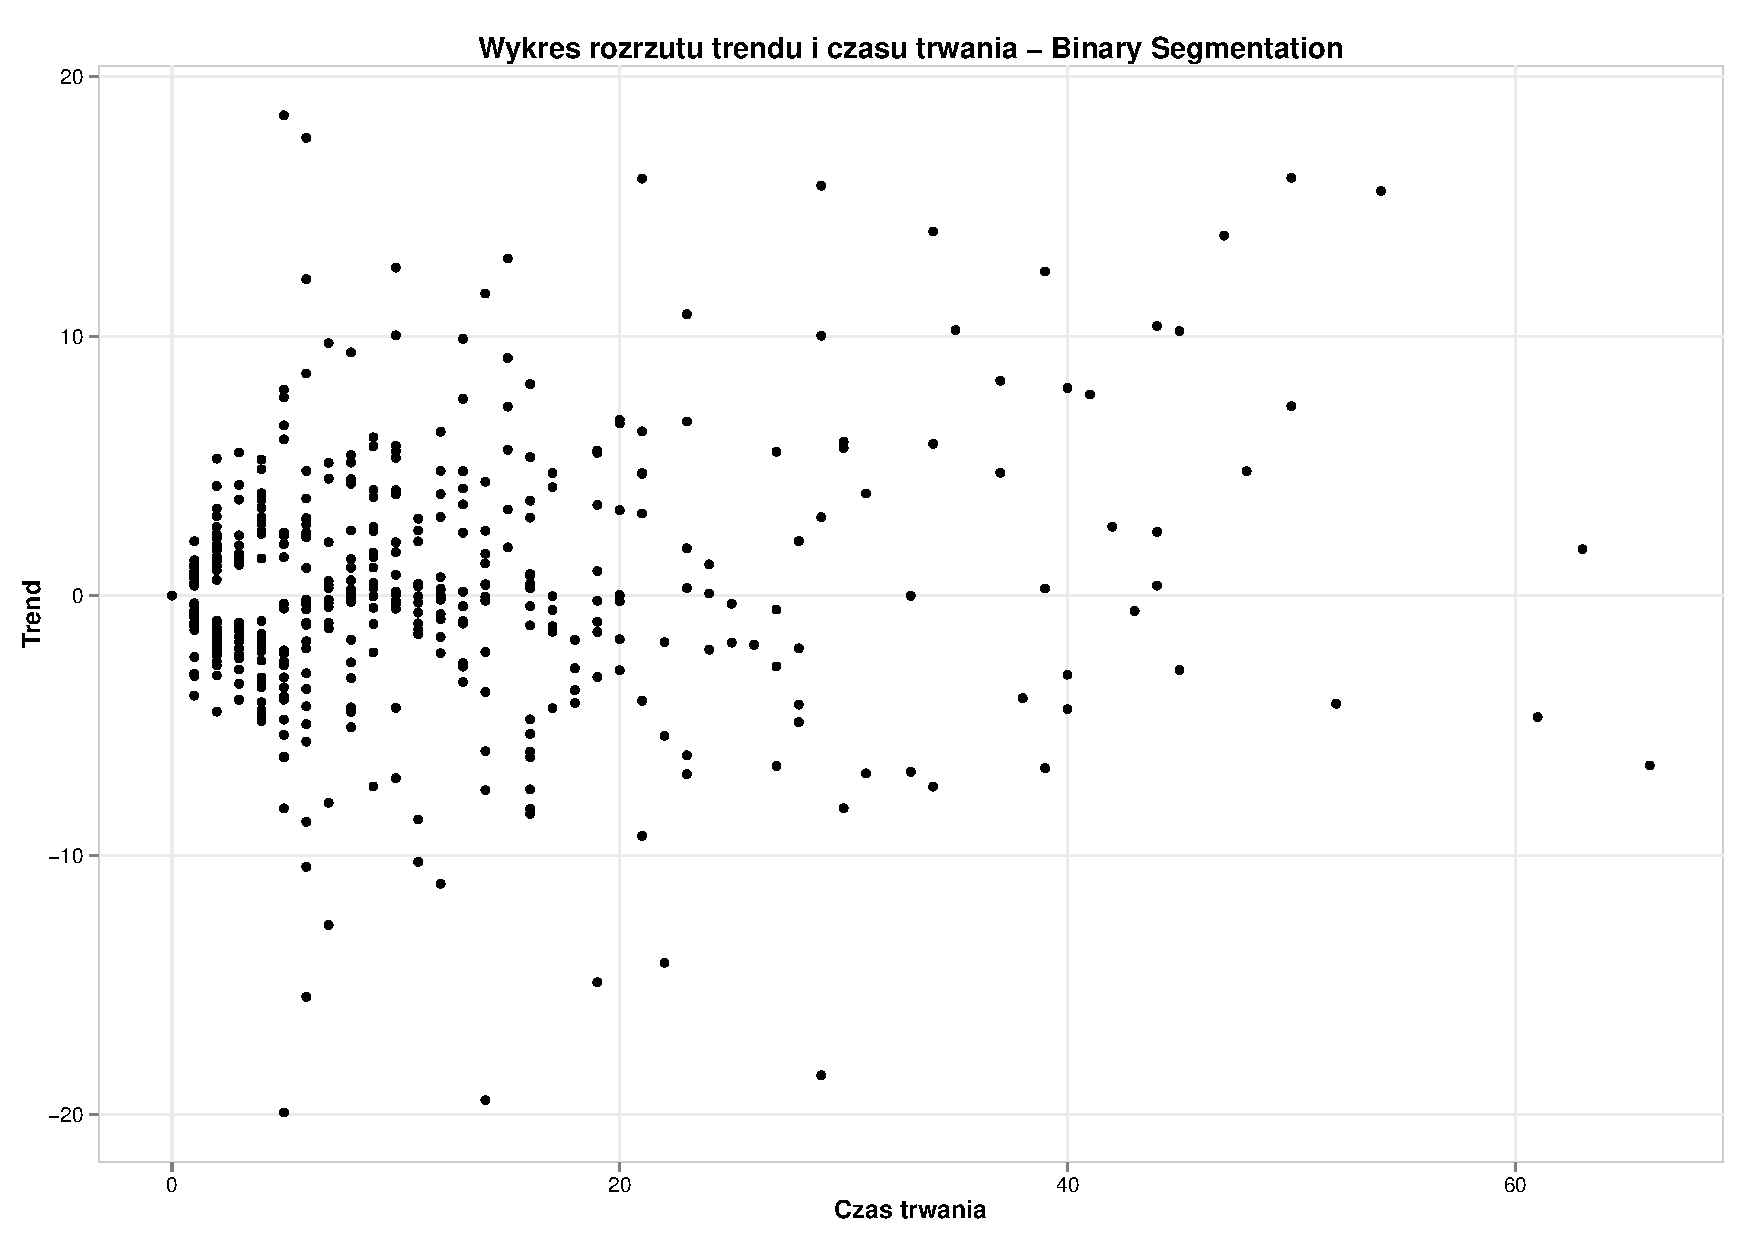
\includegraphics[width=\textwidth]{./rys010}
  \end{subfigure}

  \captionsetup{margin=10pt,font=small,labelfont=bf,width=.8\textwidth}

  \caption[Wykres rozrzutu trendu i czasu trwania dla Binary Segmentation]{Wykres rozrzutu trendu i czasu trwania dla Binary Segmentation. \textit{Źródło:} opracowanie własne}\label{rys010}
\end{figure}

\begin{figure}[H]
  \centering

  \begin{subfigure}[t]{1.00\textwidth}
    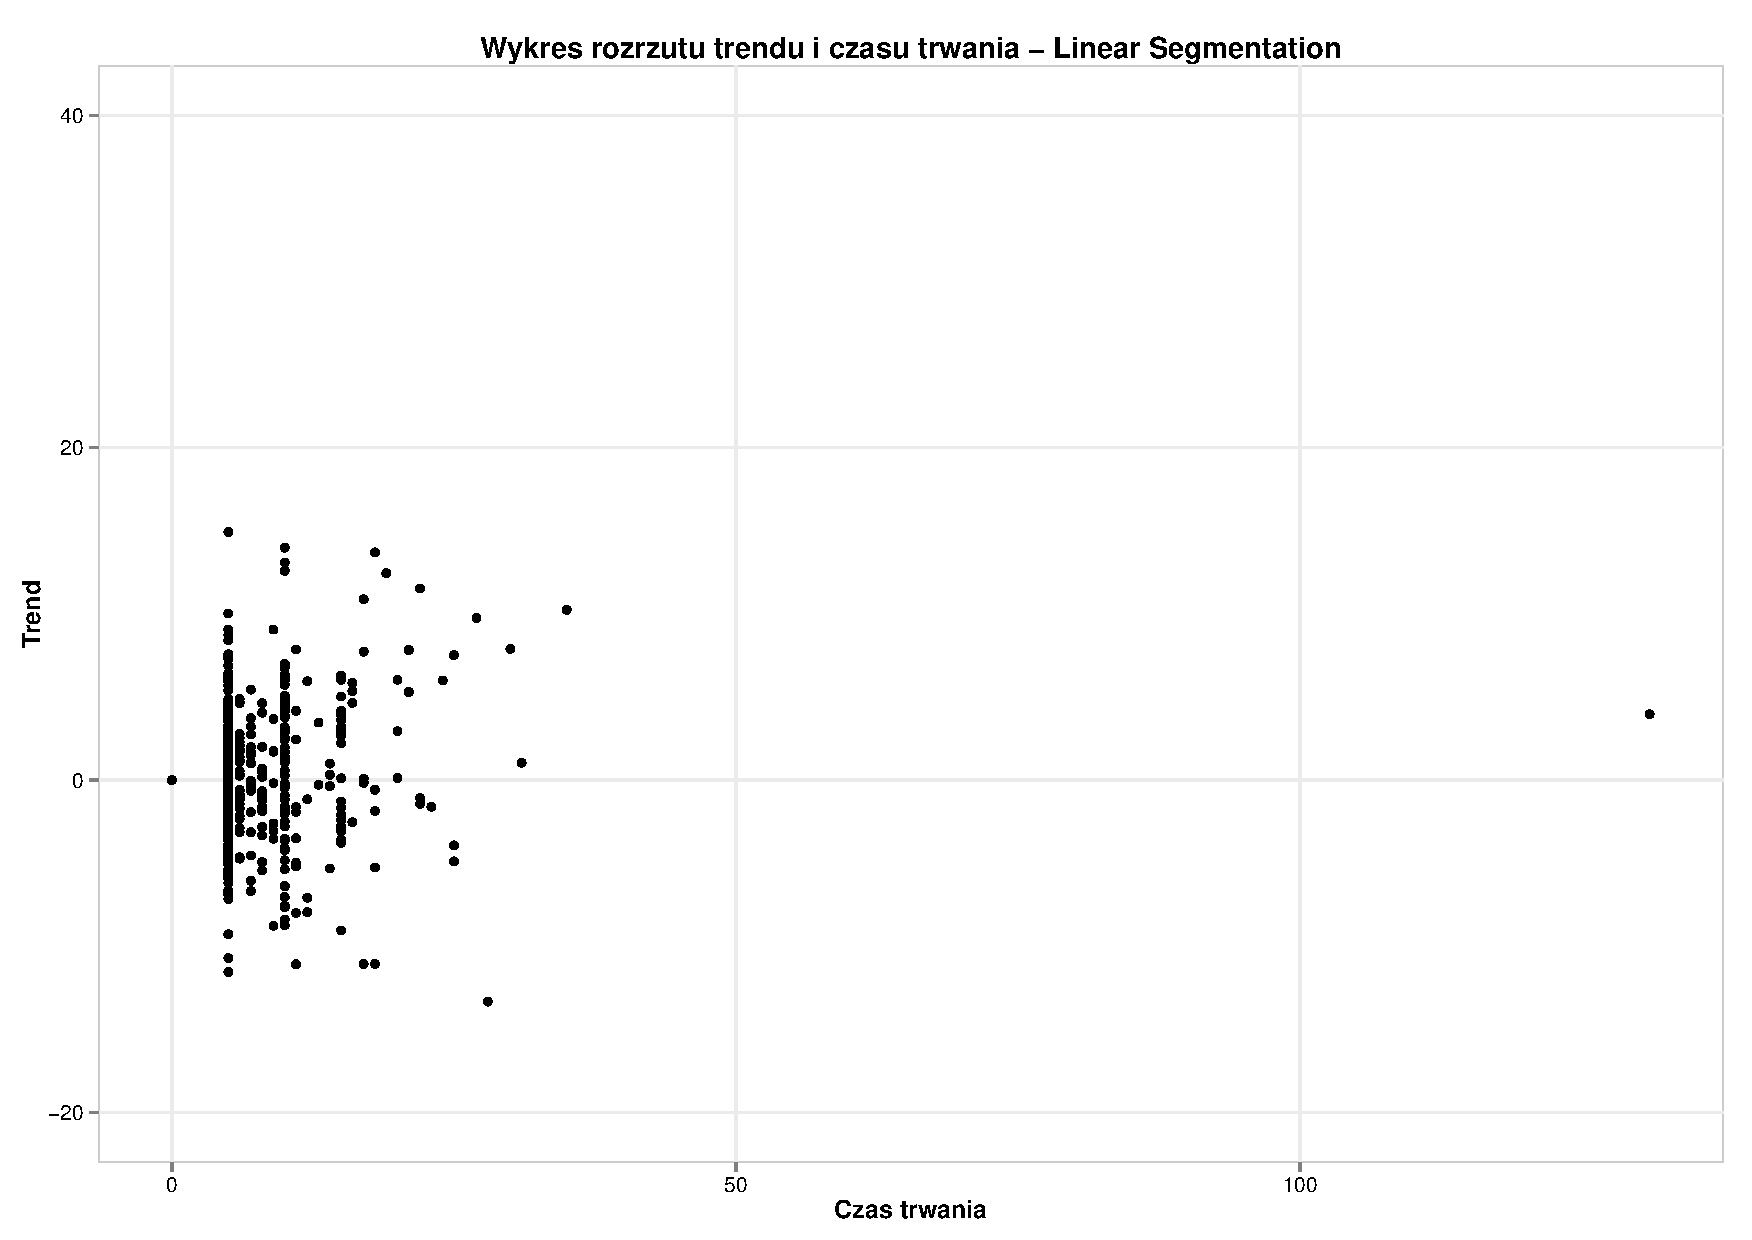
\includegraphics[width=\textwidth]{./rys011}
  \end{subfigure}

  \captionsetup{margin=10pt,font=small,labelfont=bf,width=.8\textwidth}

  \caption[Wykres rozrzutu trendu i czasu trwania dla Linear Segmentation]{Wykres rozrzutu trendu i czasu trwania dla Linear Segmentation. \textit{Źródło:} opracowanie własne}\label{rys011}
\end{figure}

Jak można zauważyć, dla \(Binary Segmentation\) segmenty są bardziej równomiernie rozłożone w stosunku do \(linear Segmentation\), gdzie większość okienek skupiona jest dla czasu trwania 
pomiędzy 5-10 dni. To sugrowałoby większą ilość klas dla metody dzielącej szereg w miejscach istotnej zmiany średniej. Graficzną reprezentację klastrowania użytego do wyznaczenia odpowiednich 
klas przedstawia wykres~\ref{rys012} oraz \ref{rys013}.

\begin{figure}[H]
  \centering

  \begin{subfigure}[t]{1.00\textwidth}
    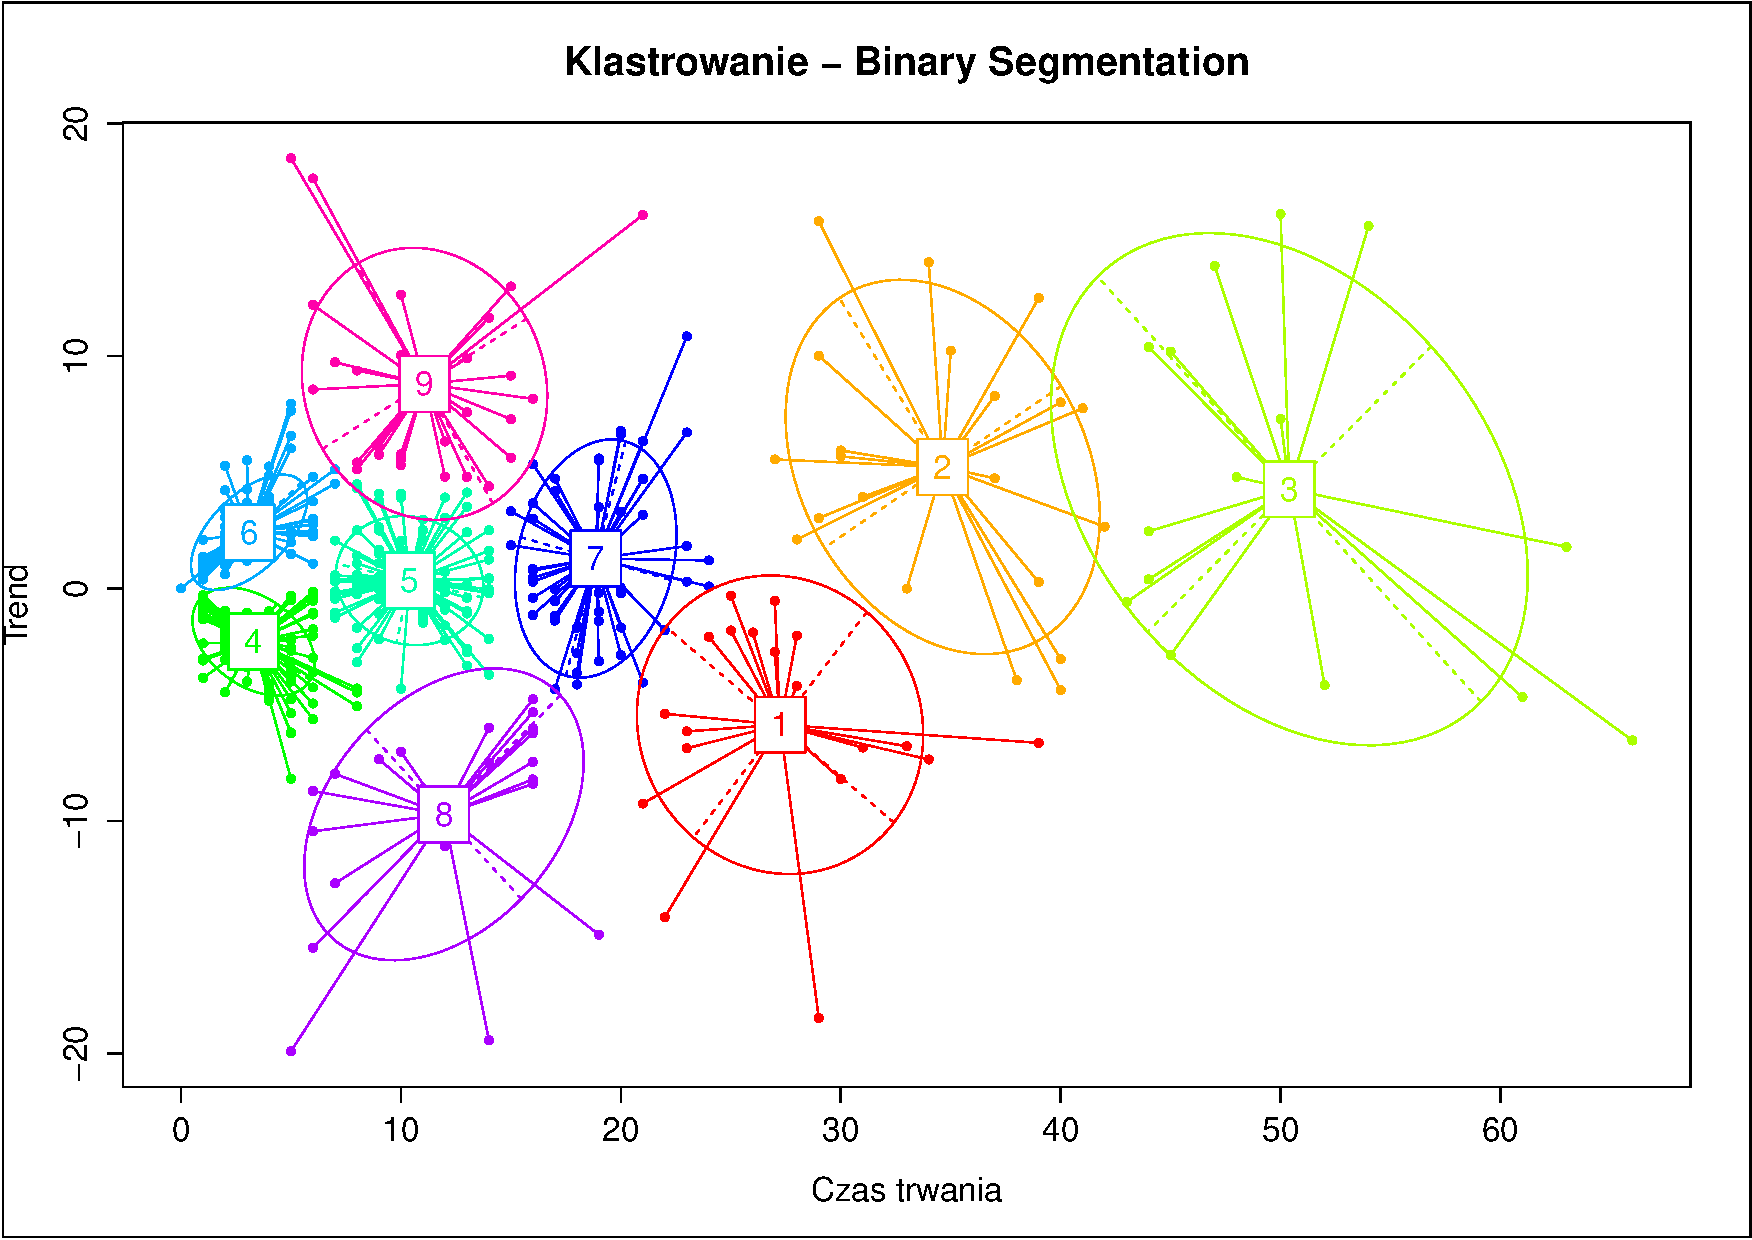
\includegraphics[width=\textwidth]{./rys012}
  \end{subfigure}

  \captionsetup{margin=10pt,font=small,labelfont=bf,width=.8\textwidth}

  \caption[Graficzna reprezentacja klastrowania dla Binary Segmentation]{Graficzna reprezentacja klastrowania dla Binary Segmentation. \textit{Źródło:} opracowanie własne}\label{rys012}
\end{figure}

\begin{figure}[H]
  \centering

  \begin{subfigure}[t]{1.00\textwidth}
    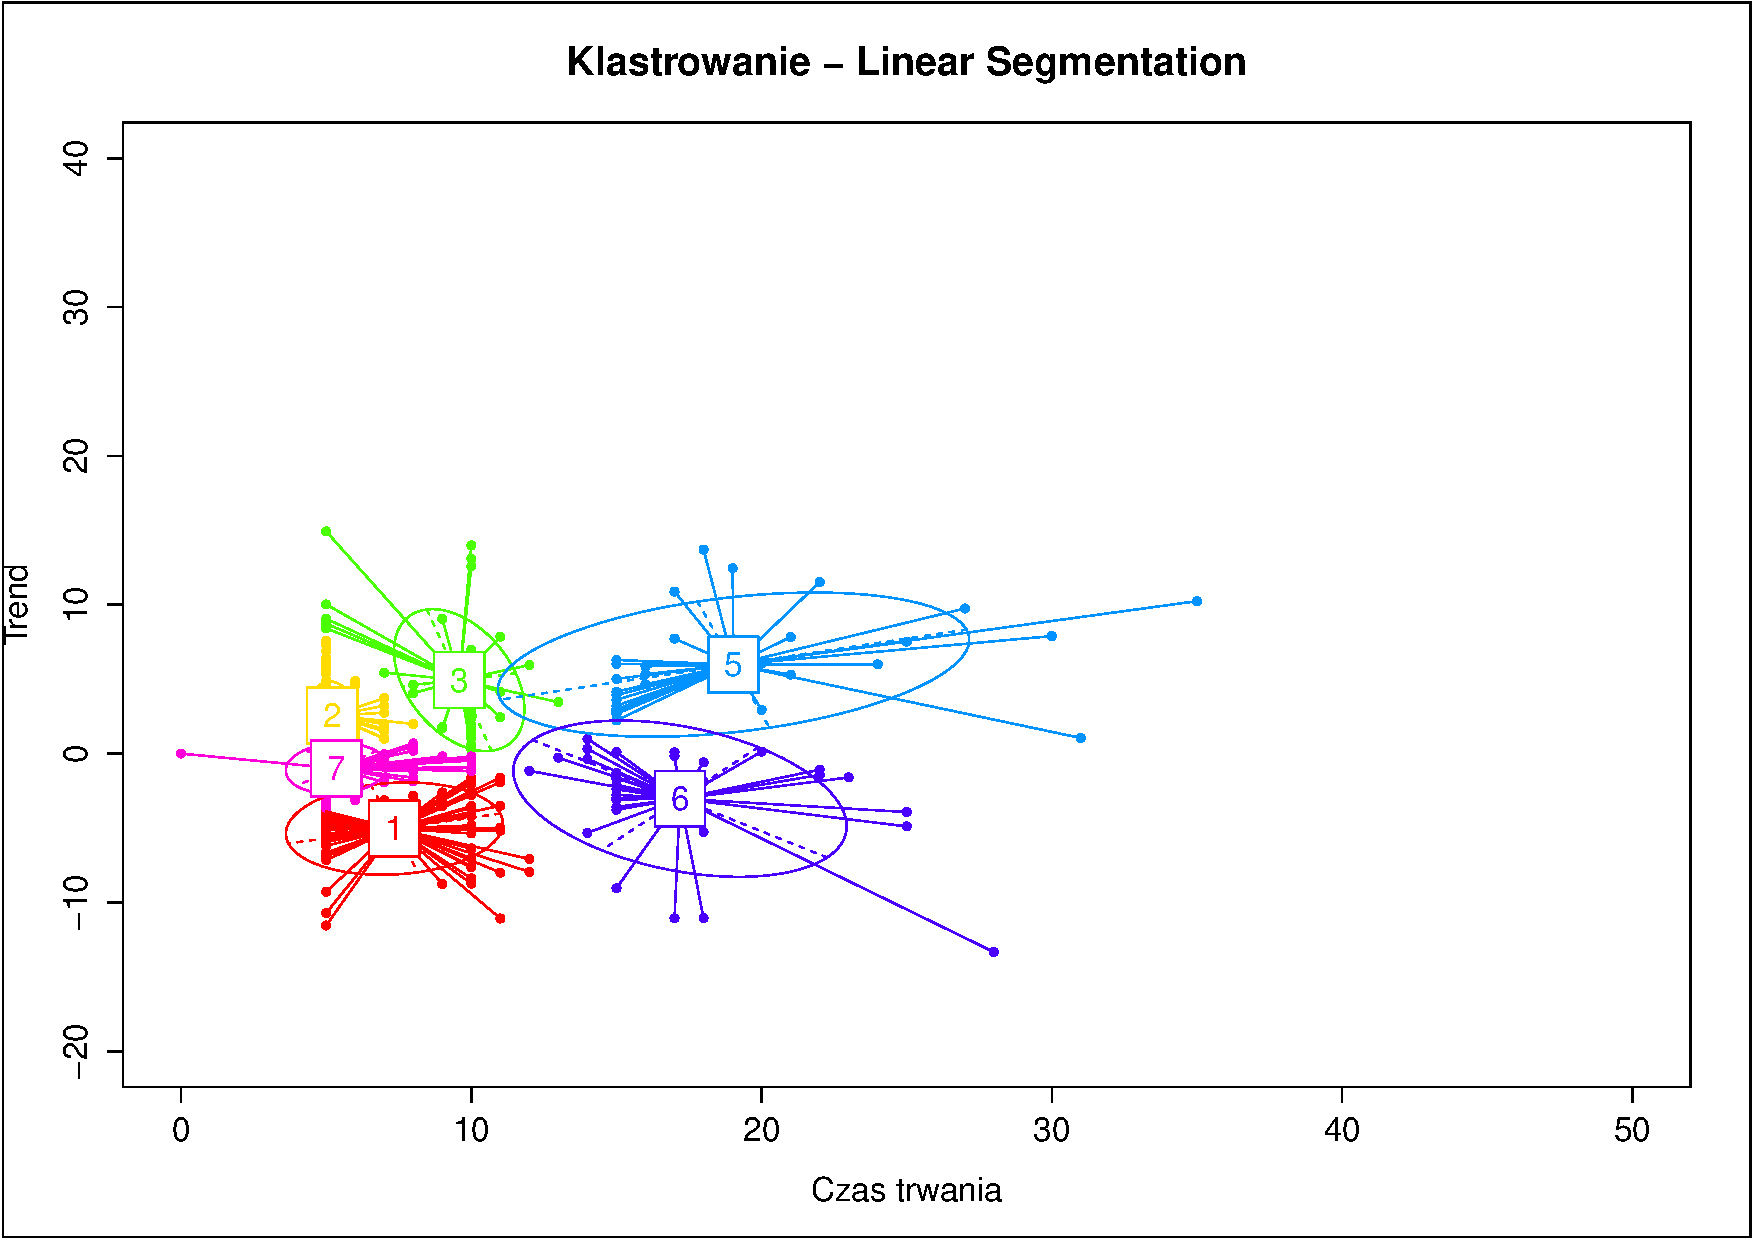
\includegraphics[width=\textwidth]{./rys013}
  \end{subfigure}

  \captionsetup{margin=10pt,font=small,labelfont=bf,width=.8\textwidth}

  \caption[Graficzna reprezentacja klastrowania dla Linear Segmentation]{Graficzna reprezentacja klastrowania dla Linear Segmentation. \textit{Źródło:} opracowanie własne}\label{rys013}
\end{figure}

\subsection{Wygenerowanie reguł asocjacyjnych}

Ostatnim krokiem przed wyznaczeniem reguł asocjacyjnych jest podział szeregu na zbiór treningowy oraz zbiór testowy, w celu późniejszej oceny użytego algorytmu. Gdy mamy 
do czynienia z dużym zbiorem danych, około 50\%-75\% obserwacji przypisujemy do próby uczącej, a reszte do testowej. Najczęściej jednak zbiór testowy stanowi mniej niż 1/3 całej próby.

W naszym przypadku, segmenty wyznaczone metodą \(Binary Segmentation\) stanowią o 36\% mniej liczny zbiór w porównaniu do okienek wyznaczonych funkcją \(linearSegmentation\)
(453 w stosunku do 700). Dlatego też dla pierwszej metody dokonujemy podziału zbioru w taki sposób, że zbiór treningowy zawiera 80\% obserwacji, natomiast testowy 20\%. Na próbie 
treningowej stosujemy algorytm Apriori, dokonując selekcji tylko tych reguł, których pewność jest większa niż \(0.5\). Ze względu na stosunkowo małą liczebność zbioru (362 obserwacje), 
dana asocjacja musi pojawić się co najmniej 3 razy. Wyniki otrzymanych reguł przedstawia tabela~\ref{tab005}.

Jak można zauważyć, ze względu na to, że klastry zawierające klasy 4 oraz 6 stanowiły najliczniejsze zbiory segmentów, dlatego też głównie one są składnikami wyznaczonych reguł.

Przykładowo, asocjacja nr. 2 stanowi, że segmenty o krótkim okresie trwania, z lekko negatywnym trendem, a następnie o długim okresie czasu (ok. 20-30 dni) z trendem wyraźnie 
spadkowym (do -20\%),  najczęściej zwiastują około 2 tygodniowy okres na rynku o trendzie horyzontalnym.

Asocjacja nr. 11 natomiast implikuje, że krótkoterminowe trendy spadkowe są powodowane przez sekwencje trzech segmentów: segmentu o czasie trwania pomiędzy ok. 7-20 dni z 
trendem wyraźnie wzrostowym (do 20\%), krótkoterminowego trendu wzrostowego (0-5\%), oraz segmentu o czasie trwania ok.10 dni z trendem horyzontalnym.

\begin{table}[H]
\caption{Reguły wyznaczone za pomocą metody Binary Segmentation. \textit{Źródło:} opracowanie własne}
\label{tab005}
\begin{tabular}{llrrr}
Lp. & Reguła & Wsparcie & Pewność  \\ 
  \hline
1 & \{lag-2=kl\_2,lag-1=kl\_6\} =$>$ \{lag0=kl\_6\} & 0.01 & 0.50  \\ 
2 & \{lag-2=kl\_4,lag-1=kl\_1\} =$>$ \{lag0=kl\_7\} & 0.01 & 0.60  \\ 
3 & \{lag-2=kl\_4,lag-1=kl\_8\} =$>$ \{lag0=kl\_4\} & 0.02 & 0.60  \\ 
4 & \{lag-2=kl\_8,lag-1=kl\_4\} =$>$ \{lag0=kl\_4\} & 0.02 & 0.70  \\ 
5 & \{lag-2=kl\_9,lag-1=kl\_6\} =$>$ \{lag0=kl\_5\} & 0.01 & 0.50  \\ 
6 & \{lag-2=kl\_5,lag-1=kl\_5\} =$>$ \{lag0=kl\_4\} & 0.02 & 0.60  \\ 
7 & \{lag-2=kl\_5,lag-1=kl\_4\} =$>$ \{lag0=kl\_4\} & 0.04 & 0.61  \\ 
8 & \{lag-2=kl\_4,lag-1=kl\_6\} =$>$ \{lag0=kl\_6\} & 0.01 & 0.75  \\ 
9 & \{lag-2=kl\_4,lag-1=kl\_4\} =$>$ \{lag0=kl\_4\} & 0.08 & 0.51  \\ 
10 & \{lag-3=kl\_4,lag-2=kl\_8,lag-1=kl\_4\} =$>$ \{lag0=kl\_4\} & 0.01 & 0.67 \\ 
11 & \{lag-3=kl\_9,lag-2=kl\_6,lag-1=kl\_5\} =$>$ \{lag0=kl\_4\} & 0.01 & 0.60 \\ 
12 & \{lag-3=kl\_6,lag-2=kl\_9,lag-1=kl\_6\} =$>$ \{lag0=kl\_6\} & 0.01 & 0.60 \\ 
13 & \{lag-3=kl\_5,lag-2=kl\_5,lag-1=kl\_4\} =$>$ \{lag0=kl\_4\} & 0.01 & 0.67 \\ 
14 & \{lag-3=kl\_5,lag-2=kl\_4,lag-1=kl\_4\} =$>$ \{lag0=kl\_4\} & 0.02 & 0.57 \\ 
15 & \{lag-3=kl\_6,lag-2=kl\_5,lag-1=kl\_5\} =$>$ \{lag0=kl\_4\} & 0.01 & 0.60 \\ 
16 & \{lag-3=kl\_4,lag-2=kl\_5,lag-1=kl\_6\} =$>$ \{lag0=kl\_6\} & 0.01 & 0.50 \\ 
17 & \{lag-3=kl\_4,lag-2=kl\_5,lag-1=kl\_4\} =$>$ \{lag0=kl\_4\} & 0.01 & 1.00 \\ 
18 & \{lag-3=kl\_4,lag-2=kl\_4,lag-1=kl\_6\} =$>$ \{lag0=kl\_6\} & 0.01 & 0.75 \\ 
19 & \{lag-3=kl\_4,lag-2=kl\_4,lag-1=kl\_4\} =$>$ \{lag0=kl\_4\} & 0.04 & 0.53
\end{tabular}
\end{table}

Dla liniowej segmentacji, ze względu na większą ilość wyznaczonych segmentów, zbiór treningowy będzie zawierał 66\% obserwacji (462 segmenty), natomiast zbiór testowy 
33\% (238 segmenty). Również w tym przypadku minimalną pewność reguł ustawiamy na \(0.5\), natomiast minimalne pojawienie się asocjacji zwiększamy do 5 razy. Wyniki 
przedstawia tabela~\ref{tab006}. 

Jak i poprzednio, najbardziej liczne klasy powstałe w wyniku klastrowania stanowią największą część składową utworzonych reguł asocjacyjnych.

Analizując strukturę wyznaczonych asocjacji, można zauważyć, że przewidywania dotyczą całkowicie tylko dwóch klas (segmentów do 10 dni o trendzie lekko wzrostowym bądź spadkowym). 
Przykładowo reguła nr. 7 określa, że 2 segmenty o lekkim trendzie spadkowym (do -2\%) oraz jeden o silniejszej tendencji spadkowej (do -10\%) poprzedzają segment ponownie 
o lekkim trendzie spadowym.


\begin{table}[H]
\caption{Reguły wyznaczone za pomocą funkcji linearSegmentation. \textit{Źródło:} opracowanie własne}
\label{tab006}
\begin{tabular}{llrrr}
Lp. & Reguła & Wsparcie & Pewność  \\ 
  \hline
1 & \{lag-2=kl\_5,lag-1=kl\_7\} =$>$ \{lag0=kl\_7\} & 0.01 & 0.62  \\ 
2 & \{lag-2=kl\_2,lag-1=kl\_3\} =$>$ \{lag0=kl\_2\} & 0.01 & 0.55  \\ 
3 & \{lag-2=kl\_2,lag-1=kl\_2\} =$>$ \{lag0=kl\_2\} & 0.08 & 0.57  \\ 
4 & \{lag-2=kl\_2,lag-1=kl\_7\} =$>$ \{lag0=kl\_7\} & 0.06 & 0.59  \\ 
5 & \{lag-3=kl\_3,lag-2=kl\_7,lag-1=kl\_7\} =$>$ \{lag0=kl\_7\} & 0.01 & 0.83  \\ 
6 & \{lag-3=kl\_1,lag-2=kl\_1,lag-1=kl\_7\} =$>$ \{lag0=kl\_7\} & 0.01 & 0.56  \\ 
7 & \{lag-3=kl\_7,lag-2=kl\_7,lag-1=kl\_1\} =$>$ \{lag0=kl\_7\} & 0.01 & 0.50  \\ 
8 & \{lag-3=kl\_2,lag-2=kl\_2,lag-1=kl\_2\} =$>$ \{lag0=kl\_2\} & 0.04 & 0.53  \\ 
9 & \{lag-3=kl\_7,lag-2=kl\_2,lag-1=kl\_2\} =$>$ \{lag0=kl\_2\} & 0.02 & 0.79  \\ 
10 & \{lag-3=kl\_2,lag-2=kl\_2,lag-1=kl\_7\} =$>$ \{lag0=kl\_7\} & 0.02 & 0.53  \\ 
11 & \{lag-3=kl\_7,lag-2=kl\_2,lag-1=kl\_7\} =$>$ \{lag0=kl\_7\} & 0.03 & 0.80  \\ 
12 & \{lag-4=kl\_2,lag-3=kl\_2,lag-2=kl\_2,lag-1=kl\_2\} =$>$ \{lag0=kl\_2\} & 0.02 & 0.53  \\ 
13 & \{lag-4=kl\_2,lag-3=kl\_2,lag-2=kl\_2,lag-1=kl\_7\} =$>$ \{lag0=kl\_7\} & 0.02 & 0.91  \\ 
14 & \{lag-4=kl\_2,lag-3=kl\_2,lag-2=kl\_7,lag-1=kl\_7\} =$>$ \{lag0=kl\_7\} & 0.01 & 0.50  \\ 
15 & \{lag-4=kl\_7,lag-3=kl\_2,lag-2=kl\_2,lag-1=kl\_2\} =$>$ \{lag0=kl\_2\} & 0.01 & 0.55  \\ 
16 & \{lag-4=kl\_7,lag-3=kl\_7,lag-2=kl\_2,lag-1=kl\_2\} =$>$ \{lag0=kl\_2\} & 0.01 & 0.75  \\ 
17 & \{lag-4=kl\_7,lag-3=kl\_2,lag-2=kl\_7,lag-1=kl\_7\} =$>$ \{lag0=kl\_7\} & 0.02 & 0.58  \\ 
18 & \{lag-4=kl\_7,lag-3=kl\_7,lag-2=kl\_2,lag-1=kl\_7\} =$>$ \{lag0=kl\_7\} & 0.02 & 0.89  \\ 
19 & \{lag-4=kl\_7,lag-3=kl\_7,lag-2=kl\_7,lag-1=kl\_7\} =$>$ \{lag0=kl\_7\} & 0.02 & 0.53 
\end{tabular}
\end{table}

\subsection{Ocena algorytmu}

Oceny jakości algorytmu dokonujemy na próbie testowej, wyszukując lewych stron wcześniej wygenerowanych asocjacji, a następnie sprawdzając czy kolejny element pokrywa się 
z prawą stroną reguły. W kolejnym kroku wyliczany jest współczynnik dokładności, w celu weryfikacji skuteczności przewidywania. Rezultaty dla obu metod przedstawiają tabele~\ref{tab007} 
oraz \ref{tab008}.

Wyniki wskazują na dużo lepsze wyniki dla asocjacji otrzymanych funkcją \(linearSegmentation\). Łącznie, dla wszystkich reguł współczynnik dokładności wynosi \(0.5466667\), co przy średniej 
pewności reguł równej \(0.6363175\) pozwala stwierdzić, że zbiór ten przeszedł pozytywnie sprawdzian krzyżowy.

 Dla segmentacji binarnej na pierwszy rzut oka widać niską liczbę pojawienia 
się reguł na zbiorze testowym. Wynika to z jego małej liczebności (91 segmenty). Aż 8 na 19 reguł nie wystąpiło w próbie, dlatego też współczynnik dokładności dla wszystkich asocjacji 
wynosił \(0.3\), podczas gdy średnia pewność dla reguł wynosiła \(0.6239613\). Na tej podstawie możemy stwierdzić, że wygenerowane asocjacje nie przeszły sprawdzianu krzyżowego. 

\begin{table}[H]
\caption{Ocena jakości algorytmu dla segmentów wyznaczonych metodą Binary Segmentation. \textit{Źródło:} opracowanie własne}
\label{tab007}
\begin{tabular}{rrrr}
Nr reguły & Prawidłowo zaklasyfikowane & Łączna liczba pojawień & Wspolczynnik dokładności \\ 
  \hline
1 & 0.00 & 0.00 &  \\ 
 2 & 0.00 & 1.00 & 0.00 \\ 
 3 & 0.00 & 0.00 &  \\ 
 4 & 1.00 & 1.00 & 1.00 \\ 
 5 & 1.00 & 2.00 & 0.50 \\ 
 6 & 0.00 & 5.00 & 0.00 \\ 
 7 & 1.00 & 2.00 & 0.50 \\ 
 8 & 0.00 & 0.00 &  \\ 
 9 & 1.00 & 3.00 & 0.33 \\ 
 10 & 0.00 & 0.00 &  \\ 
 11 & 0.00 & 1.00 & 0.00 \\ 
 12 & 0.00 & 0.00 &  \\ 
 13 & 0.00 & 0.00 &  \\ 
 14 & 1.00 & 1.00 & 1.00 \\ 
 15 & 0.00 & 1.00 & 0.00 \\ 
 16 & 1.00 & 2.00 & 0.50 \\ 
 17 & 0.00 & 0.00 &  \\ 
 18 & 0.00 & 0.00 &  \\ 
 19 & 0.00 & 1.00 & 0.00 
\end{tabular}
\end{table}

\begin{table}[H]
\caption{Ocena jakości algorytmu dla segmentów wyznaczonych za pomocą funkcji linearSegmentation. \textit{Źródło:} opracowanie własne}
\label{tab008}
\begin{tabular}{rrrr}
Nr reguły & Prawidłowo zaklasyfikowane & Łączna liczba pojawień & Wspolczynnik dokładności \\ 
  \hline
1 & 4.00 & 5.00 & 0.80 \\ 
 2 & 4.00 & 6.00 & 0.67 \\ 
 3 & 13.00 & 25.00 & 0.52 \\ 
 4 & 13.00 & 20.00 & 0.65 \\ 
 5 & 2.00 & 3.00 & 0.67 \\ 
 6 & 0.00 & 4.00 & 0.00 \\ 
 7 & 2.00 & 10.00 & 0.20 \\ 
 8 & 7.00 & 13.00 & 0.54 \\ 
 9 & 4.00 & 8.00 & 0.50 \\ 
 10 & 8.00 & 11.00 & 0.73 \\ 
 11 & 2.00 & 3.00 & 0.67 \\ 
 12 & 3.00 & 7.00 & 0.43 \\ 
 13 & 5.00 & 6.00 & 0.83 \\ 
 14 & 4.00 & 8.00 & 0.50 \\ 
 15 & 2.00 & 4.00 & 0.50 \\ 
 16 & 3.00 & 5.00 & 0.60 \\ 
 17 & 1.00 & 2.00 & 0.50 \\ 
 18 & 2.00 & 2.00 & 1.00 \\ 
 19 & 3.00 & 8.00 & 0.38
\end{tabular}
\end{table}

\clearpage
\section{Podsumowanie}

Podsumowując rozważania na temat powyższego algorytmu można stwierdzić, że wydobywanie reguł asocjacyjnych z finansowych szeregów czasowych jest procesem 
wieloetapowym i złożonym. Wymaga ono odpowiedniego przygotowania i obróbki danych, zanim będzie możliwe jakiekolwiek wyciąganie wniosków na przyszłość. Jak jednak 
wskazują wyniki, zaproponowany powyżej algorytm, użyty do indeksu giełdowego WIG20, daje niezadowalające rezultaty. Mimo, że zbiór obserwacji wydaje się być duży (5235 obserwacji), 
niemożliwe jest wygenerowanie reguł zawierających większą liczbę segmentów, a przez to łatwiej interpretowalnych i podobnych do formacji znanych z analizy technicznej.

Dla segmentów wyznaczonych za pomocą funkcji dzielącej szereg w miejscach istotnej statystycznie zmiany średniej wyniki są niesatysfakcjonujące, ponieważ zbiór testowy jest zbyt mały, by było 
możliwe zweryfikowanie czy wyznaczone reguły decyzyjne potrafią poprawnie prognozować na danych nieużytych przy ich generowaniu. Problem może więc leżeć w tym, że 
funkcja binarnej segmentacji jest zbyt danochłonna i właściwe byłoby jej użycie dla dłuższych szeregów czasowych. Ograniczenie tej metody może wynikać także z niewłaściwego 
doboru odpowiedniej ilości klastrów, przez co niektóre obserwacje mogą być pomijane stosując algorytm Apriori, ponieważ liczebność danego klastra będzie zbyt mała. Niewątpliwym 
atutem tego podejścia jest fakt, że powstałe segmenty cechują się różnorodną charakterystyką, mniejszym skupieniem, a przez to prowadzą do powstania bardziej zróżnicowanych 
reguł decyzyjnych.

Jeśli chodzi o wyniki dla okienek wyznaczonych za pomocą metody liniowej segmentacji, są one poprawne pod względem sprawdzianu krzyżowego, jednak wyznaczone reguły 
niosą ze sobą małą wartość informacyjną, ze względu na to że ich składowe stanowią praktycznie wyłącznie dwie klasy. Problem stanowi więc tutaj charakterystyka segmentów 
wyznaczanych za pomocą tej metody. Tak jak wcześniej zostało stwierdzone, większość z nich jest długości równej tej podanej w argumencie funkcji. To powoduje, że algorytm 
klastrowania wyznacza 2 zbiory, które w przeciwieństwie do pozostałych charakteryzują się obecnością dużej liczby obserwacji, a to w konsekwencji prowadzi do uwzględniania 
tylko ich stosując algorytm Apriori. Plusem tej metody jest duża liczba segmentów, pozwalająca na jednoznaczne określenie przydatności prognostycznej asocjacji.

Biorąc więc pod uwagę wszystkie powyższe wnioski, możliwe jest ulepszenie zaproponowanego algorytmu, tak aby otrzymać korzystniejsze rezultaty. Można tego dokonać na 
etapie segmentacji szeregu, stosując inną metodę, bądź na etapie odpowiedniego podziału segmentów, używając np.: kryterium Calinski-Harabasz do określenia właściwej liczby 
klastrów. Również zaaplikowanie innego algorytmu do wyznaczania reguł asocjacyjnych (np. algorytm Eclat) mogłoby przynieść pozytywny efekt.

% --- appendices ------------------------------------------------------
\appendix


\clearpage
\section{Dodatek: Tabela współczynników wielomianu kwadratowego dla filtra Savitzky'ego-Golaya}
Jako że współczynniki dopasowania wielomianu są symetryczne (\(a_{i}=a_{-i}\)), tabela ta zawiera tylko współczynniki dla elementów nieujemnych. \\
\begin{table}[h]
\begin{tabular}{rrrrrrrrrrrrrrr}
NP & H & \(a_{0}\) & \(a_{1}\) & \(a_{2}\) & \(a_{3}\) & \(a_{4}\) & \(a_{5}\) & \(a_{6}\) & \(a_{7}\) & \(a_{8}\) & \(a_{9}\) & \(a_{10}\) & \(a_{11}\) & \(a_{12}\)  \\ \hline
5 & 35 & 17 & 12 & -3 & 0 & 0 & 0 & 0 & 0 & 0 & 0 & 0 & 0 & 0 \\
7 & 21 & 7 & 6 & 3 & -2 & 0 & 0 & 0 & 0 & 0 & 0 & 0 & 0 & 0 \\
9 & 231 & 59 & 54 & 39 & 14 & -21 & 0 & 0 & 0 & 0 & 0 & 0 & 0 & 0 \\
11 & 429 & 89 & 84 & 69 & 44 & 9 & -36 & 0 & 0 & 0 & 0 & 0 & 0 & 0 \\
13 & 143 & 25 & 24 & 21 & 16 & 9 & 0 & -11 & 0 & 0 & 0 & 0 & 0 & 0 \\
15 & 1105 & 167 & 162 & 147 & 122 & 87 & 42 & -13 & -78 & 0 & 0 & 0 & 0 & 0 \\
17 & 323 & 43 & 42 & 39 & 34 & 27 & 18 & 7 & -6 & -21 & 0 & 0 & 0 & 0 \\
19 & 2261 & 269 & 264 & 249 & 224 & 189 & 144 & 89 & 24 & -51 & -136 & 0 & 0 & 0 \\
21 & 3059 & 329 & 324 & 309 & 284 & 249 & 204 & 149 & 84 & 9 & -76 & -171 & 0 & 0 \\
23 & 805 & 79 & 78 & 75 & 70 & 63 & 54 & 43 & 30 & 15 & -2 & -21 & -42 & 0 \\
25 & 5175 & 467 & 462 & 447 & 422 & 387 & 343 & 287 & 222 & 147 & 62 & -33 & -138 & -253 
\end{tabular}
\end{table}

% ---------------------------------------------------------------------
\clearpage
\section{Dodatek: Kod R}

\lstinputlisting{./praca_lic_skrypt_bpz.R}


% --- bibliography ----------------------------------------------------
\clearpage
\bibliographystyle{agsm}
\bibliography{refs}

% --- abstract --------------------------------------------------------
\clearpage
\addcontentsline{toc}{section}{Lista tablic}
\listoftables

% --- abstract --------------------------------------------------------
\clearpage
\addcontentsline{toc}{section}{Lista rysunków}
\listoffigures



% --- abstract --------------------------------------------------------
\clearpage
\addcontentsline{toc}{section}{Streszczenie}
\section*{Streszczenie}

Niniejsza praca przedstawia własny algorytm do wyznaczania reguł asocjacyjnych z finansowych szeregów czasowych, pozwalający na prognozowanie przyszłych ruchów cen. Algorytm 
został zastosowany dla indeksu giełdowego WIG20. Zawiera narzędzia statystyczne oraz używane w data mining'u i składa się z 5 kroków. Pierwszy krok stanowi czyszczenie danych z nadmiaru 
krótkoterminowych wahań i używa do tego celu filtr Savitzky'ego-Golaya. Drugim krokiem jest segmentacja szeregu na fragmenty o podobnej charakterystyce. Od tego momentu algorytm 
jednocześnie przeprowadzany jest dla dwóch metod (segmentacja liniowa oraz binarna), w celu porównania ich działania. Trzecim krokiem jest zbudowanie słownika, tzn. przypisanie segmentów o 
podobnej charakterystyce do odpowiednich klas. Czwarty etap to zastosowanie algorytmu Apriori do wyznaczenia reguł asocjacyjnych, natomiast ostatni to ocena ich własności prognostycznej, 
dzięki podziałowi zbioru na próbę treningową i testową. Wyniki powyższego schematu postępowania okazują się być niezadowalające, dlatego też sugerowana jest odpowiednia modyfikacja algorytmu.

\end{document}
